%%
%% Beuth Hochschule für Technik -- Bachelorarbeit
%%
%% Hauptdokument
%%
%--------------------------------------------------------------%

\documentclass[11pt, a4paper,parskip=half]{report}
\usepackage[abgabe]{bhtThesis}
\typeout{Bachelorarbeit}

\usepackage{graphicx}
\usepackage{hyperref}

\usepackage{blindtext}
\usepackage{listings}
\usepackage{color}

\lstset{
	literate =	{ö}{{\"o}}1
				{ä}{{\"a}}1
				{ü}{{\"u}}1
				{Ö}{{\"O}}1
				{Ä}{{\"A}}1
				{Ü}{{\"U}}1
				{ß}{{\ss}}1
}
\usepackage{trsym}
\usepackage{bytefield}
\usepackage{longtable}
\definecolor{light-gray}{gray}{0.90} %Code Hintergundfarbe

%Pfad zu den Bildern
\graphicspath{
	{pictures/},
	{einleitung/pictures/},
	{5_Systementwurf/pictures/}
}

\definecolor{darkBHT}{rgb}{0,0.5882,0.5529}
\setlength{\parskip}{6pt}
\setlength{\parindent}{0pt}

\definecolor{lightgray}{rgb}{.9,.9,.9}
\definecolor{darkgray}{rgb}{.4,.4,.4}
\definecolor{purple}{rgb}{0.65,0.12,0.82}

%format for program code
\lstset{language=C++,
				backgroundcolor=\color{white},
				%frame=single,
				tabsize=2,
				numbers=left,
				numbersep=0pt,
				basicstyle=\ttfamily\color{black}\small,
				keywordstyle=\color{HKS51}\bfseries,
				commentstyle=\color{HKS13}\slshape,,
				identifierstyle=\color{black}
		}


\begin{document}

\pagestyle{fancy}


\begin{titlepage}
	\begin{center}
		\Large
		Beuth Hochschule für Technik Berlin
		\textcolor{darkBHT}{\rule{\textwidth}{0.2cm}} \\
		\vspace{2 cm}
		\Huge
		\textbf{Bachelorarbeit}
		\vspace{2 cm}
		
		\begin{figure}[htbp]
			\centering 
			
\includegraphics[width=9cm]{BHT-Logo-Basis.pdf}  
		\end{figure}
		
		\vspace{3cm}
		\Large
		WN Serial COM Port Tester\\
		\vspace{3cm}
		\begin{tabular}{lcl}
			Erstprüfer:& &Prof. Dr. Voß\\
			Zweitprüfer:& &Prof. Dr. Görlich\\
		\end{tabular} 
		\\
		\vspace{0.8cm}
		Eingereicht am \\
		\today % Aktuelles Datum
		\vspace{0.8cm}
		
		Eingereicht von \\
		\begin{tabular}{ll}
			Matthias Hansert & 764369\\
		\end{tabular}

	\end{center}
	\vfill
	\textcolor{darkBHT}{\rule{\textwidth}{0.2cm}}
	\vspace{1 cm}
	\normalsize
	
\end{titlepage}

%
% EOF
%

\pagenumbering{Roman}
\tableofcontents %Inhaltsverzeichnis
%one empty page after table of contents
\newpage
\thispagestyle{empty}
\mbox{}
\newpage
\thispagestyle{empty}
\mbox{}

%--------------------------------------------------------------%
% Die Kapitel
%--------------------------------------------------------------%
\pagenumbering{arabic}
\chapter{Einleitung}
hgdjkgfjkshgfkhjsagjhlfhaklshfklafjkajksfhjkadshjklfgadjklfga
sadfasjhdfghjkasgdhjkfgahjksdgfhjasgjlhfgajsfjlhasd
SDGFSAJKFGJKHASDGFHJKASGHJKFGAHJKSDFGHJASGHDF
.asdhjgshjkafghjkasfcachvlkwklr tekluwthkerhköaenkfgae

\chapter{Aufgabenstellung}\label{chp:aufgabenstellung}
\paragraph{}
Das Tool soll die RS-232 Schnittstelle testen und die Schwächen der vorhandenen Lösungen ergänzen. Die Firma Wincor Nixdorf besitzt derzeit schon ein Tool welches die Druckertestumgebung testet, dies ist aber auf Ruby basierend. Das Programm "`WN Serial COM Port Tester"' soll mit Funktionsaufrufen der WinAPI programmiert werden. Die aktuell vorhandenen Lösungen, wie zum Beispiel das Programm "`AGGsoft Serial Port Tester"' haben eingeschränkte Einstellungen und sind nicht ausführlich genug für die Voraussetzungen der Qualitätssicherung.

\section{Module}
\paragraph{}
Das Programm bietet dem Nutzer folgende Schnittstellen an um es zu bedienen:
\begin{itemize}
\item Windows-GUI(Graphical User Interface) mit allen Einstellmöglichkeiten und Start-Button.
\item Kommandozeilen User Interface mit passenden Einstellmöglichkeiten, wie auch per GUI und Rückgabewerte (Exitcodes).
\item Funktionskern, der aus beiden UI angesprochen wird und die eigentlichen Tests durchführt.
\end{itemize}


\section{Laufzeit}
\paragraph{}
Das Com-Port-Test Programm kann von einem schreibgeschütztem Medium (z.B. Windows-PE-CD) laufen, d.h. alle Schreibfunktionen (Log-Datei) sind per Option abschaltbar. Die Testparameter können in einer Konfigurationsdatei gespeichert und wieder geladen werden. Alle Ereignisse und Meldungen können in einer Log-Datei eingetragen werden. 

Wenn das Programm mit einem Skript ausgeführt wird startet das Com-Port-Test Programm und testet die Ports automatisch. Unter Ports sind die im die BEETLE Systeme eingebaute COM Ports zu verstehen. Solche Ports sind Legacy oder durch PCI erweiterbare Ports.


\section{Hardware}
\paragraph{}
Folgende Hardware-Kombinationen werden unterstützt (die Reihenfolge hier gibt die Priorität der Implementierung wieder):
\begin{enumerate}
\item Test einer Schnittstelle mit Kurzschlussstecker auf einem System
\item Test zweier Schnittstelle mit Null-MODEM-Kabel (RxD/TxD gekreuzt; RTS/CTS gekreuzt, etc.) auf einem System
\item Test zweier Schnittstelle mit Null-MODEM-Kabel auf unterschiedlichen Systemen! Siehe dazu auch „Synchronisierungsprotokoll“…
\end{enumerate}



\section{Betriebssystem}
\paragraph{}
Das Programm "WN Serial COM Port Tester" ist für folgende Zielbetriebssysteme entwickelt worden:
\begin{itemize}
\item Windows XP SP3 x86, x64; Windows 7 x86, x64; WinPE 2.x (WinXP) / 3.x (Win7)
\item Windows 8 nur ein Test, der aussagt ob es kompatibel ist oder noch etwas zu tun wäre
\end{itemize}
Linux - Distributionen werden vom Programm nicht unterstützt.

\section{Logbuch}
\paragraph{}
Alle Ereignisse und Testschritte können zu Dokumentations- und Analysezwecken in einer Log-Datei gespeichert werden. Auch Fehler, die der Parser in der Test-Datei(.ini) findet, werden in der Log-Datei eingetragen. Der Name der Log-Datei ist für jede Instanz und jedes Testsystem eindeutig zu wählen, wie im folgenden Beispiel zu sehen ist:
\\
\\ \hspace*{10mm}<Programmname>\_<Computername>\_<Master/Slave>\_<Port>.csv

\paragraph{}
Jeder Eintrag bekommt einen Uhrzeit und Datums-Stempel. Eine Zeile sieht dann wie folgt aus:
\\
\\ \hspace*{10mm} <Datum>; <Uhrzeit>;<Ereignis>;<Wert>;<Kommentar>

\paragraph{}
Die ersten beiden  Einträge der Log-Datei:
\\
\\ \hspace*{10mm} <Datum>; <Uhrzeit>;START;RS232-Port-Nummer; INI-Dateiname als Kommentar



\section{Programminstanzen}
\paragraph{}
Das Programm kann in mehrfachen Programm-Instanzen gestartet werden, in der Regel läuft bei umfangreichen Tests für jeden zu testenden RS-232-Port eine Programm-Instanz. Das vermeidet aufwändige Thread-Programmierung eines einzigen Programms für alle Ports. Das ist keine feste Vorgabe, der Entwickler kann entscheiden welcher Lösungsweg  als geeignet befindet.

\textbf{würde ich nochmal umschreiben zu umgangssprachlich -> alt...} Das ist keine feste Vorgabe, sollte sich Thread-Programmierung als einfacher erweisen, dann sollte es auch benutzt werden.


\section{Master / Slave}
\paragraph{}
Jede Programminstanz wird als Master, Slave oder mit beiden Konfigurationen gestartet.


\subsection{Master-Funktion}
\paragraph{}
Im Master-Modus schickt die Schnittstelle die vorgegebenen Texte / Dateien mit den eingestellten Parametern an den Slave. Der Master wertet die dem Test zugeordnete INI-Datei aus, der Slave folgt nur dem Master. Der Master wartet auf das Echo oder auf eine Fehlermeldung und bewertet den Testschritt sobald der Test komplett und fehlerfrei empfangen worden ist. Zugleich bewertet er ob der Test erfolgreich oder fehlerhaft war. In beiden Fällen werden Fehler, Warnungen und Erfolgsmeldungen geloggt.


\subsection{Slave-Funktion}
\paragraph{}
Im Slave-Modus (Programminstanz auf gleichem System oder zweiten BEETLE/PC)werden die Daten komplett empfangen, wertet eventuelle Fehler aus und schickt entweder die Daten als Echo oder eine Fehlermeldung wieder zurück. 

\subsection{Master / Slave Kombination mit Kurzschlussstecker}
\paragraph{}
Im kombinierten Master / Slave-Modus (Kurzschlussstecker) übernimmt eine Instanz des Programms beides, das heißt, sie schickt sich selber Daten und antwortet ebenso. Programm intern laufen aber die beiden Module (Master / Slave) weitestgehend getrennt ab.

\subsection{Master / Slave Ablauf mit „Wobbeln“-Funktion}
\paragraph{}
Die Master-Instanz übernimmt die Steuerung des Ablaufes, der Slave antwortet dem Master. In diesem Testmodus werden durch den Benutzer eingegebene Baudraten(Unter und Obergrenze) gewobbelt. Der Wobbeln-Ablauf kann über die GUI oder in der INI-Datei beschrieben werden. Der automatische Test erfolgt dann nur für die dort eingetragenen Parameter, z.B.:

\begin{center}
BAUD = 9600 - 115200
\end{center}
\paragraph{}
Hier werden die Baudrate von 9600 bis 115200 für den Test berücksichtigt, aber 2400, 300, etc. weiter nicht. Wenn mehrere Parameter flexibel gesetzt / programmiert sind, werden alle Kombinationen getestet. Das kann dann durchaus eine nicht unerhebliche Testzeit beanspruchen.
\paragraph{}
Die Programminstanz öffnet die zugehörige Schnittstelle automatisch mit der ersten von allen der programmierten Optionen (Baudrate, Parität, etc.) und startet dann einen Testdurchlauf mit diesen Einstellungen. Wenn alle Daten fehlerfrei gesendet und danach auch das Echo fehlerfrei empfangen wurden,  wird der Port geschlossen, mit der nächsten Kombination geöffnet und wieder Daten gesendet und empfangen. Wenn Fehler (Parität, Offline, etc.) vom Master erkannt oder vom Slave gesendet wurden, dann wird der letzte Schritt wiederholt. Jedes Lese- oder Schreibvorgang wird fünf mal versucht. Wenn der aktuelle Test schon die x-te Fehler-Wiederholung war, dann stoppt das Programm und zeigt den Fehler an. Dieser Fehler-Zustand darf durch das Programm nicht verändert werden. Der Tester / Entwickler muss die Fehler analysieren.

\subsection{Synchronisierungsprotokoll}
\paragraph{}
Für den Wobbelmodus ist ein minimales Protokoll zur Synchronisation nötig. Wenn eine Programminstanz als Master gestartet wird, erhält sie die nötigen Schnittstellenparameter per GUI oder aus der Konfigurationsdatei. Sie sendet diese in From eines Konfigurationspakets dem Slave. Solche Konfigurationspakete werden immer mit den Standardschnittstellenparametern (96,o,8,1) gesendet. Der Slave synchronisiert sich dann, d.h. programmiert -per WIN-API- seinen zu testenden Port mit den empfangenen Parametern und wartet auf Nutzdaten.
\paragraph{}
Wenn der erste Test erfolgreich war (Master hat gesendet und der Slave hat ein Echo geschickt), dann schickt der Master an den Slave die Parameter des nächsten Testschritts. Das ist nötig, weil im Fehlerfall (Echo fehlerhaft empfangen) der Slave nicht mehr synchron wäre, er weiß nur ob seine Daten fehlerfrei gesendet wurden, aber nicht ob der Empfang richtig angekommen ist. Der Slave kann so einfach nur mit Standard-Parametern gestartet werden und folgt dann dem Master.


\section{Teststruktur}
\paragraph{}
Gefordert ist eine einfache Trennung von Testablauf / Testoptionen  und  Testobjekt(RS-232-Port). Die Teststeuerung wird daher sowohl im Programm selber, als auch über die Kommandozeile implementiert. Der Testablauf für jeden Port selber ist in der zugehörigen Konfigurationsdatei vollständig, aber unabhängig vom zu testenden Port (RS-232-Port / V.24-Schnittstelle), beschrieben. Es können mehrere Konfigurationsdateien auf der Kommandozeile übergeben werden. Die Schnittstellenummer wird über die Kommandozeile festgelegt. So kann der gleiche Testablauf (INI-Datei) für jeden Port einzeln oder parallel durchgeführt werden.


\section{Benutzerschnittstelle}

\subsection{GUI}
\paragraph{}
In der GUI sind alle Programm- und Schnittstellenparameter einstellbar und können jederzeit aus der GUI in eine Konfigurationsdatei gespeichert werden. Das Windows-Fenster bietet also implizit auch die Funktion eines Konfigurationseditors mit eingebauter Syntaxüberprüfung.


\subsection{Kommandozeile}
\paragraph{}
Wenn die Kommandozeile keine Parameter bekommt, wird automatisch die GUI dargestellt. Die Kommandozeile nimmt folgende Optionen entgegen:
\begin{itemize}
\item -f INI\_Datei
\item -f INI\_Datei /Port
\end{itemize} 
In der INI Datei ist der Testvorgang beschrieben. Wenn kein "/Port"' angegeben wurde, dann wird der Port in der INI Datei getestet. So sieht ein Programmaufruf aus:
\begin{itemize}
\item SerialPortTester.exe KOMPLETT.INI
\item SerialPortTester.exe KOMPLETT.INI /COM3 
\end{itemize} 

\section{Skriptfähigkeit}
\paragraph{}
Per Kommandozeile gestartet, ist das Programm BATCH-/Script-fähig, d.h. es startet ohne weitere Benutzereingaben, loggt alle Ereignisse und auch Hinweise -zur Analyse nach dem Test- in die zugehörige Datei und beendet sich ebenso selbstständig. Fehler, Warnungen und Hinweise werden auf der Konsole ausgegeben. Als Option kann es auch im Hintergrund ohne jede Anzeige laufen.


\section{Programmierung der Testparameter}
\paragraph{}
Die Testparameter können direkt per GUI oder per INI-Datei eingestellt werden. Die aktuelle Testkonfiguration und der Ablauf kann in einer INI-Datei gespeichert und wieder geladen werden. Eine mit GUI erstellte INI-Datei kann über die Kommandozeile geladen werden. Diese INI-Datei hat die Windows-übliche Struktur mit „[“ und „]“ und ist per Notepad (oder anderen Editor) editierbar.
\\
Sie enthält alle Informationen zur Steuerung der Programminstanz, dass heißt alle einstellbaren Schnittstellenparameter inklusive Wobbelnoption (von-bis):
\begin{tabbing}
\hspace*{10mm}Baudrate = 1200-9600; \=Stopbbits = 1; Datenbits = 8; RTS\_CTS=yes; etc.
\\
\hspace*{10mm}Baudrate = min-max; \>Stopbbits = min-max; etc.
\end{tabbing}

Für MIN/MAX siehe Schnittstellenoptionen. Timeout-Werte (für Echo-Antworten auf Datenpakete) sollten keine festen Zeiten programmiert sein, das Programm  berechnet die Wartezeiten automatisch aus der aktuellen Baudrate. Verzögerungszeiten zwischen zwei Datenblöcken/Testschritten inklusive Zufallswert ist wünschenswert.


\subsection{Schnittstellenoptionen zu Test}
\paragraph{}
Folgende Werte sollen für den Benutzer einstellbar sein:

\begin{itemize}
\item Baudrate
\item Parität
\item Datenbits
\item Stopbits
\item Flusssteuerung
\end{itemize}
\paragraph{}
Das Programm kann hier mit Variablen MIN und MAX umgehen. Wenn beispielsweise die Zeile „BAUDRATE = MAX“ oder „BAUDRATE = MIN“  programmiert wurde,  sucht das Programm die maximale bzw. minimale Baudrate, die angegebene RS-232-Port unterstützt und nutzt sie für den Test. Diese Werte werden aus „dem System“ –beispielsweise Registry oder  MSPORTS.DLL direkt ausgelesen. Manuell können diese MIN/MAX-Werte über den Gerätemanager ermittelt werden. Wenn keine Parameter übergeben wurden, startet das Programm mit diesen Standardparametern: 9600,odd,8,1,RTS/CTS (von der Wincor Nixdorf Anzeige BA66).

\paragraph{}
Die Wobbelnoption wird in Form einer VON-BIS-Zeile implementiert:

\begin{tabbing}
\hspace*{10mm} BAUDRATE=300;2400;9600;115200 \= diese vier Werte werden getestet
\\
\hspace*{10mm} BAUDRATE=MIN-MAX \>alle möglichen Werte
\\
\hspace*{10mm} BAUDRATE=300-9600;115200 \>alle Werte von 300 bis 9600 und 115200 im Test
\end{tabbing}


\subsection{Sendedaten aus Datei}
\paragraph{}
Als Testdaten werden feste Texte (in der Regel ASCII Zeichen) oder auch Pattern aus einer Datei gesendet. Die Dateipfade / Sendetexte sind als Testparameter in der GUI oder Test-Datei) einstellbar. Wenn keine Sendedaten übergeben wurde, dann sendet das Programm zufällige, aber auf einem Protokollanalysator lesbare, ASCII-Zeichen: 0x20 ... 0x7F .


\section{Fehlererkennung und Behandlung}
\paragraph{}
Folgende mögliche Fehlerfälle muss ein solches Tool erkennen:
\begin{itemize}
\item Kabel-/Stecker-Fehler („Wackelkontakt“ durch schlechten mechanischen Kontakt Stecker/Buchse) 
\item Elektrische Fehler, die sich bei Übertragung über langes Null-MODEM-Kabel im Form von Paritäts-, Rahmenfehlern oder ähnliches zeigen
\item Dauerhaft gezogene Kabel / Kurzschlussstecker
\item Windows-interne Ressourcenprobleme (Shared Interrupts)
\end{itemize} 
\paragraph{}
Bei Erkennung eines Übertragungsfehlers wird dieser in die Logdatei eingetragen und / oder auf der Konsole angezeigt und danach der letzte Block wiederholt. Nach der x-ten erfolglosen Wiederholung (Wert aus Test-Datei) erfolgt Testabbruch

%%%%%%%%%%%%%%%%%%%%%%%%%%%%%%%%%%%%%%%%%%%%%%%%%%%%%%%%%%%%
\newpage
%%%%%%%%%%%%%%%%%%%%%%%%%%%%%%%%%%%%%%%%%%%%%%%%%%%%%%%%%%%%

\section{Neue Anforderungen}
\subsection{Logbuch}
\paragraph{}
Der Name der Logdatei soll im eine Nummer erweitert werden. Wenn eine Logdatei auf das Zielsystem schon vorhanden sein, wird die Nummer hochgezählt.\\

\hspace*{10mm}<Programmname>\_<Computername>\_<Master/Slave>\_<Port>\_<Nummer>.ini

Wenn der Test direkt über GUI-Optionen konfiguriert wurde, dann werden diese Werte in eine INI-Datei vor dem Teststart gesichert und diese in der Logdatei eingetragen.

\subsection{Synchronisierungsprotokoll}
\paragraph{}
Das erste solcher Konfigurationspakete wird immer mit den Standardschnittstellenparametern (96,o,8,1) gesendet. Ein solches Paket beginnt mit einem Fluchtzeichen (in ASCII wäre das ESCAPE 0x1B) und wird vom Slave per Bestätigungszeichen (in ASCII ACK) beantwortet.


\subsection{Anhalten eines Tests}
\paragraph{}
Will der Benutzer ein Test vorzeitig beenden, gibt es eine Schaltfläche auf der GUI die der Test anhaltet. Wird per Kommandozeile das Programm ausgeführt, kann der Benutzer durch das drücken der "`ESC"' Taste ein Test stoppen.
\chapter{Fachlichesumfeld}
\section{Dast ist eine Section}
\subsection{Das ist eine SubSection}
\subsubsection{Das ist eine SubSubSection}
\newpage
\section{Dast ist eine Section}
\subsection{Das ist eine SubSection}
\subsubsection{Das ist eine SubSubSection}
\chapter{Lösungsansätze}\label{chp:loesungsansaetze}

\section{Fehlererkennung}
\paragraph{}
Das Ziel des COM-Port-Test-Programm ist Fehler in der Systemhardware, beziehungsweise in der Kommunikation zwischen den Schnittstellen zu erkennen. Damit dieses Ziel erreicht wird, muss die Ermittlung eines Fehlers äußerst genau geschehen. So muss jeder Funktionsaufruf und Kommunikationsvorgang immer abgefragt werden. Bei jeder Abfrage müssen die Fehler ausgewertet und gemeldet werden. Nur so erfüllt das Testprogramm seinen Zweck. Die Herausforderung wird darin bestehen, die Fehler genau zu definieren und sie so zu melden, dass der Tester die Ursache sofort erkennen kann.

\section{Master Slave Modus zwischen zwei Systemen}
\paragraph{}
Die Synchronisierung zwischen zwei verschiedenen BEETLE Systemen wird eine große Herausforderung darstellen. Dafür wird ein kleines Protokoll oder Handshake definiert. In diesem Vorgang muss der Master wissen, dass der Slave fertig eingestellt und bereit für ein Datenverkehr ist. Dabei müssen beide Schnittstellen die richtige Einstellungsparameter (Baudrate, Paritätbits, Stopbits, Datenbits, etc.) besitzen und konfigurieren.\\


Um das Protokoll oder Handshake zu definieren gibt es verschiedene Möglichkeiten. Zusätzlich müssen zuerst die Timeouts beachtet werden. Der Master darf keine Information oder Übertragungstexte senden, bevor der Slave nicht in der Lage ist, Daten zu empfangen. Wäre der Slave nicht bereit sein, würde der Master ein Lese-Timeout melden, weil er Daten verschickt hat, aber der Empfänger keine Daten zurück versendet. Im Gegensatz, darf der Slave nicht Daten erwarten, so lange der Master nicht in der Lage ist, Daten zu verschicken.\\


Als Grundidee, um dieses Problem zu lösen, werde ich Synchronisierungszeiten und Vorgänge einbauen, in dem der Master für eine definierte Zeit auf den Slave wartet. Wenn diese Zeit abgelaufen ist, wird dem Benutzer gemeldet, dass es Probleme mit der Synchronisierung beider Systeme gab und dass kein Test stattfinden wird. Ein großer Nachteil dieser Lösung ist, dass durch das Abfragen auf Bereitschaft ein Pollingverfahren\footnote{Das zyklische Abfragen eines Status} eingesetzt werden muss. \\


Im besten Fall, wenn keine Fehler bei der Kommunikation auftreten, wird es nicht so nötig sein, sich ständig zu Synchronisieren. Im Fehlerfall muss nach jedem Test eine Synchronisierung stattfinden. Empfängt der Slave verfälschte Informationen und meldet einen Fehler, wurde er sich sofort auf den nächsten Test vorbereiten. Das würde den gesamten Testvorgang verfälschen. Es werden weitere solche Fälle auftreten, auf die unterschiedlich  reagiert werden muss.\\


Um das Pollingverfahren zu vermeiden, kann die Synchronisierung auf Basis von Events \footnote{http://msdn.microsoft.com/en-us/library/aa450667.aspx; 30.08.2013} basieren. Dabei erzeugt die Schnittstelle bei der Ankunft von einem Byte Interrupts. So kann der Slave reagieren, erst wenn der Master tatsächlich etwas verschickt hat. Um die Interrupts abzufragen, muss die Kommunikation Events von Windows abfragen. Wenn das System ein Interrupt empfängt, wird dieses im Programm als Event weitergeleitet.\\


Auf den ersten Blick wird das vollkommene Umgehen eines Pollingverfahrens schwer sein. Die Lösung wird sich durch Tests während der Entwicklung des "WN Serial COM Port Tester" ergeben. Je nach Testergebnis werde ich unterschiedliche Lösungen anwenden.



\section{C++ und die GUI}\label{C++GUILoesung}
\paragraph{}
Die graphische Oberflächen mit Anwendung von der Windows API besteht aus "`C"' Code, und muss eine statische Fensterprozedur besitzen. Das heißt, es können beliebig viele Benutzeroberflächen kreiert werden, aber es gibt nur eine Prozedur, die die Nachrichten bearbeitet. Durch die Objektorientierung unter "`C++"' ersteht ein Konflikt wegen der statischen Fensterprozedur. Um eine statische Methode zu definieren, müssen auch statische Variablen erzeugt werden. So werden diese Variablen nur einmal erzeugt, unabhängig davon, wie viele Fenster erstellt werden. Wenn die Methoden und die Variablen nicht statisch wären, würden bei der Ersetllung von mehreren Fenstern die versendeten Nachrichten durcheinander kommen.\\


Um dieses Problem zu umgehen wird mit Hilfe von einer \textit{Template Class} die Oberfläche definiert. Eine Klasse wird definiert, in der die allgemeinen Eigenschaften eines Fensters gesetzt werden und die Nachrichten von jedem Fenster richtig umgeleitet werden. Dieses geschieht indem die benötigte statische Fensterprozedur in dem Template definiert wird. Die allerersten Nachrichten, die ein Programm erhält, um eine Oberfläche zu erzeugen, ist die "`WM\_NCREATE"'. Die Fensterprozedur fragt nach dieser Nachricht und wenn die Nachricht ankommt, wird durch einen Zeiger der Fensterhandle richtig gesetzt und an die richtige Prozedur weitergeleitet. Da diese Fensterprozedur statisch ist, egal wie viele Oberflächen kreiert werden, wird es nur einmal diese Fensterprozedur geben.\\


Die Fensterklasse erbt von der \textit{Template Class} und kann eine eigene Fensterprozedur definieren. Die definierte Fensterprozedur in der Fensterklasse wird durch das Template die Nachrichten weiterleiten. Dadurch werde ich auch in der Lage sein, meine eigene Fenster so zu gestalten wie die Voraussetzungen es definieren, und falls es nötig ist, mehrere Fenster zu erzeugen.
\chapter{Systementwurf}\label{chp:systementwurf}


\section{Klasse Window}
\paragraph{}
Die Klasse \textit{Window} baut die Benutzeroberfläche auf und speichert die Eingabe des Benutzers in Variablen. Diese Werte werden dann an die Klasse \textit{Interpreter} weiter gegeben. In der Benutzeroberfläche werden die Eigenschaften für jeden Testvorgang eingestellt.


\subsection{Design}
\begin{figure}[h]
  \begin{center}
    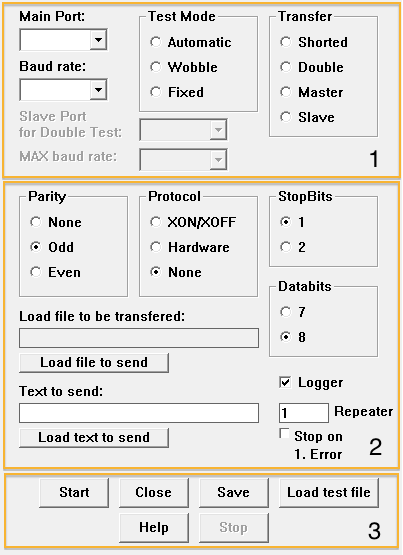
\includegraphics[scale=0.6]{gui.png}
  		  \caption{Design der Benutzeroberfläche}
     \label{GUI_Bild}
  \end{center}
\end{figure}


Die Benutzeroberfläche ist in drei Abschnitte geteilt. Die verschiedenen Abschnitte sind in der Abbildung \ref{GUI_Bild} zu erkennen. Genaueres zu alle Parametern wird in Kapitel \ref{chp:bedienungsanleitung} und  \ref{chp:fachlichesumfeld} erläutert. Der erste Abschnitt der Einstellungen behandelt die Testeinstellungen. 

\newpage

Diese Einstellung sind:
\begin{itemize}
\item Main Port: welcher COM Port soll getestet werden
\item Baud rate: beschreibt mit welcher Baudrate der ausgewählte Port getestet werden soll
\item Test Mode: definiert welchen Testvorgang der Benutzer haben möchte
\item Transfer: legt fest, wie die Kommunikation dieses Ports stattfinden wird
\end{itemize}

Der Slave Port for "`Double Test"' und "`Max baud rate"' (grau dargestellt) sind abhängig vom Testmodus und Transfermodus.\\

Der zweite Abschnitt sind die Übertragungsparameter und drei weitere Testeinstellungen. Diese Parameter sind:

\begin{itemize}
\item Parity: Paritätsüberprüfung
\item Protocol: Übertragungsprotokoll
\item Stopbits: Anzahl der Stopbits
\item Databits: Anzahl der Datenbits
\item Logger: definiert ob eine Log-Datei erstellt werden soll
\item Repeater: Anzahl der Testwiederholungen
\item Stop on 1. Error: bestimmt ob bei der ersten Fehlererkennung angehalten werden soll
\item Load file to be transfered: Übertragungsdatei die übertragen wird
\item Text to send: Übertragungstext der gesendet wird\\
\end{itemize}

Die letzte Reihe von Elementen in der Benutzeroberfläche sind die Schaltflächen. Diese führen die jeweiligen Vorgänge aus.

\begin{itemize}
\item Start: startet einen Test
\item Close: schließt das Test Tool
\item Save: speichert in eine Testdatei mit den Einstellungen
\item Load test file: lädt eine Datei die im Test übertragen wird
\item Help: zeigt ein Fenster mit Erklärungen zum Test Tool
\item Stop: stoppt den laufenden Test\\
\end{itemize}

Beim Drücken des Start-, Save- oder "`Load test file"' Schaltfläche werden die Testeinstellungen an die Klasse \textit{Interpreter} weitergegeben und dort werden diese verarbeitet.


\subsection{Aufbau}
\paragraph{}
Die Klasse \textit{Window} erbt von der \textit{Template class} in der Headerdatei \textit{BaseWindow}. Die Headerdatei beinhaltet die Definition des Templates. Im Template, wird die für die Nachrichtenschleife nötige, statische Fensterprozedur deklariert. Hier wird nur nach der Nachricht \textit{WN\_NCCREATE} abgefragt, wie bereits im Kapitel \ref{C++GUILoesung} erwähnt wurde. Wenn die Nachricht empfangen worden ist, werden die weiteren Nachrichten an das Handle des Fensterobjekts weitergeleitet. In dem Template wird außerdem auch eine Fensterklasse deklariert, registriert und danach erzeugt. Somit werden alle Nachrichten eines Fensterobjektes immer zuerst an die statische Fensterprozedur gesendet, diese leitet durch einen Zeiger und ein Handle die Nachricht an das korrekte Fenster weiter. Um genauer die Funktionalität des Templates zu verstehen, siehe bitte Anhang \ref{TemplateClass}.

\subsection{Aufgaben}
\paragraph{}
Die Klasse hinter der Benutzeroberfläche besteht aus zwei Teilen. Der erste Teil bearbeitet die Eingabe des Benutzers und den Aufbau der Oberfläche, der zweite Teil die Weiterbearbeitung der Daten.\\

Der erste Teil besteht aus der Methode \textit{HandleMessage}. Diese Methode ist die Fensterprozedur. Zuerst  werden die Elemente, mit der Ankunft der Nachricht \textit{WM\_CREATE} des Fensters aufgebaut. Danach wird auf die Nachricht \textit{WM\_COMMAND} gewartet und jeweils reagiert. Wird zum Beispiel die Start Schaltfläche gedrückt, bekommt die \textit{HandleMessage} Methode die \textit{WM\_COMMAND} Nachricht mit dem Parameter \textit{ID\_BT\_START}, das ist die Identifikationsnummer im Programm für die Startschaltfläche.\\

\begin{lstlisting}	 
	case WM_CREATE:
	{
    		//Erzeuge alle GUI Elemente
    
    		//example: Start button
		_hwnd_Start = CreateWindowA("button", "Start",
   		WS_CHILD | WS_VISIBLE,
   		POS_X + 20, POS_Y2 + 290, 70, 30, m_hwnd, (HMENU)ID_BT_START,
   		NULL, NULL);
	}
	break;
\end{lstlisting}

Wenn die Startschaltfläche gedrückt worden ist, fängt der zweite Teil der Klasse an. Der zweite Teil besteht aus der Weiterverarbeitung der Eingaben. Im Fall der Startschaltfläche, wird als erstes ein neuer Thread erzeugt. So kann die Benutzeroberfläche immer noch Nachrichten verarbeiten, während im Hintergrund das Programm die Datenverarbeitung beginnt. Der gleiche Vorgang geschieht, wenn die \textit{Load test file} Schaltfläche gedrückt wird.\\

\newpage

Wenn die Startschaltfläche gedrückt wird, ruft der Thread die Methode \textit{SendTestSettings} auf. Die Eingabe werden weiter an einen Interpreter-Objekt gegeben. Dies geschieht in dem ein Objekt der Klasse \textit{Interpreter} erzeugt wird und dessen Eigenschaften gesetzt werden.

\begin{lstlisting}	 
	case WM_COMMAND:
	{
		//Reagiere auf Klicks der Schaltfäche
		//Beispiel: Startschaltfläche
		case ID_BT_START:

			//während des Tests werden die Elemente grau hinterlegt
			viewAllElements(FALSE);

			//erzeuge ein neuen Thread
			_t1 = thread(&Window::sendTestSettings, this);

			//abtrennen des Threads für den Test, während der Mainthread
			//auf Stopp warten oder Testende
			_t1.detach();
	}
    break;
\end{lstlisting}




%****************************************************************************************
\newpage
%****************************************************************************************

\section{Klasse Interpreter}
\paragraph{}
Die Klasse \textit{Interpreter} trennt die Benutzeroberfläche von der Fachlogik des Programms. Die Benutzeroberfläche kann den Interpreter aufrufen und hat Zugriff auf die \textit{public} Methoden der Klasse. Der Interpreter kann nicht auf Elemente oder Methoden der Klasse \textit{Window} zugreifen. Durch diese Trennung kann der Benutzer nie "`unkontrolliert"' auf die Fachlogik zugreifen, nur über die Möglichkeiten die der Programmierer ihn anbietet.\\

\subsection{Aufgaben}
\paragraph{}
Eine Aufgabe des Interpreters ist die Überprüfung der Eingaben des Benutzers, bevor die Tests beginnen. Durch so genannte "`setter"'-Methoden werden die Eingabeparameter der GUI in lokalen Variablen gespeichert.\\


\begin{lstlisting}	 
	void Interpreter::setTransfer(int iTransfer)
	{
		this->_iTransfer = iTransfer;
	}
\end{lstlisting}

Danach werden die lokalen Variablen auf Fehleingaben geprüft. Sind Fehler erkannt worden, werden diese dem Benutzer bekannt gegeben und alle Parameter in der Klasse werden auf einen Standardwert zurückgesetzt. Sind keine Fehleingaben erkannt worden, werden die Werte der Variablen in einer Datenstruktur gespeichert. Mehr zu dieser Struktur wird im Kapitel ~\ref{TestStruct} behandelt. Im folgenden Quellcode wird eine Fehlerüberprüfung dargestellt, hierbei handelt es sich um den Übertragungsmodus, der abgefragt wird.

\begin{lstlisting}	 
	if (_iTransfer == DEFAULT_VALUE)
	{
		MessageBoxA(NULL,"Bitte wählen Sie ein Transfermodus aus",
                    WINDOW_TITLE, MB_OK | MB_ICONERROR);
		setDefaultValues();
	}
	else
	{
		//speichern des Transfermodus
		_testManager->testStruct.iTransfer = _iTransfer;
	}
\end{lstlisting}

Die Werte in den Variablen müssen überprüft werden, um Fehler zu vermeiden. Da die Werte nicht nur aus Einstellungen in der Benutzeroberfläche stammen, sondern auch aus einer Testkonfigurationsdatei, können falsche Eingabe vorhanden sein. Zusätzlich zur Überprüfung der Eingabeparameter und setzen der lokalen Variablen, gibt die Klasse \textit{Interpreter} die Testeinstellungen an die anderen Klassen weiter. Hier trennt sich das Programm in zwei Pfade. Der erste Pfad gibt die Datenstruktur an die Klasse \textit{TestManager} weiter. Der zweite Pfad speichert oder liest eine Testkonfigurationsdatei aus. Im Fall, dass eine Testkonfigurationsdatei gelesen werden soll, wird als erstes die Klasse \textit{IniFileHandler} aufgerufen und danach die Klasse \textit{TestManager}, um einen Test mit den gelesenen Einstellungen zu starten. Sollen die Eingabeparameter der Benutzeroberfläche in einer Testkonfigurationsdatei gespeichert werden, werden die überprüften Eingabeparameter in einer vom Benutzer angegebenen Datei gespeichert. Dafür wird auch die Klasse \textit{IniFileHandler} aufgerufen.\\

Da die Klasse \textit{Interpreter} die Schnittstelle für die Kommunikation zwischen Fachlogik und der Benutzeroberfläche ist, wird auch durch diese Klasse die Meldung gegeben, den Test anzuhalten. Durch das Klicken der Schaltfläche "`Stop"' in der Benutzeroberfläche wird eine boolesche Variable weiter an die Testlogik gegeben. Diese Variable wird vor jeder Testschleife abgefragt, ist sie gesetzt, dann wird der Test angehalten.\\

Die Klasse hat ein Objekt der Klasse \textit{Com}, um in der Benutzeroberfläche die im System zur Verfügung stehenden COM Ports aufzulisten. Durch die Trennung der GUI von der Fachlogik, darf die \textit{Window} Klasse kein Objekt der Klasse \textit{Com} haben.\\



%****************************************************************************************
\newpage
%****************************************************************************************

\section{Struktur TestStruct}\label{TestStruct}
\paragraph{}
Eine \textit{struct} oder Struktur dient dazu, mehrere logische zusammenhängende Variablen verschiedener Datentypen zusammenzufassen. In \textit{C} beinhalten Strukturen nur Variablen, in \textit{C++} wurden die Strukturen erweitert und dürfen auch Funktionen beinhalten. Der Unterschied von einer Klasse zu einer Struktur ist, dass die jeweiligen Attributen bzw. Eigenschaften mit Zugriffsrechten versehen werden können. In einer Struktur sind die Zugriffsrechte auf Elemente mit  \textit{public} definiert, in einer Klasse mit \textit{private}\footnote{\cite{VisualC++}}. Da ich nur Variablen benötige, und keine Methoden, habe ich mich für eine Struktur entschieden.


\subsection{Aufbau}
\paragraph{}
Die Datenstruktur fasst alle Eigenschaften für einem Test zusammen. Die \textit{TestStruct} beinhaltelt folgende Variablen und wird wie folgt definiert:\\

\begin{lstlisting}	 
	struct TestStruct
	{
		string sMasterPort;
		string sSlavePort;
		string sTextToTransfer;
		string sFilePath;
		int iTransfer;
		int iBaud;
		int iBaudrateMax;
		int iTestMode;
		int iParity;
		int iProtocol;
		int iStopbits;
		int iDatabits;
		int iTransTextMode;
		int iRepeater;
		bool bLoggerState;
		bool bStopOnError;
		vector<string> svBaudrates;
	}
\end{lstlisting}

Jede dieser Variablen stellt einen Wert für eine Einstellung in der Benutzeroberfläche dar. Für eine genauere Erläuterung der Variablen und dessen Werte, siehe bitte Kapitel \ref{chp:bedienungsanleitung} und \ref{IniFileHandler}.

%****************************************************************************************
\newpage
%****************************************************************************************


\section{Klasse Com}
\paragraph{}
Die Klasse \textit{Com} umfasst alles für die Verwaltung eines COM Ports. Um aus einem COM Port lesen und schreiben zu können, müssen zuerst die Eigenschaften des jeweiligen Ports gesetzt werden. Alle Ports in einem System werden beim Systemstart mit einer Standardkonfiguration konfiguriert. Will der Benutzer Peripherieelemente an einem COM Port anschließen, die nicht die gleiche Schnittstellenkonfiguration besitzen wie die Schnittstelle im System, muss die Konfiguration des Ports angepasst werden. Dafür muss ein COM Port zuerst geöffnet werden, danach kann die Konfiguration geändert werden. Wenn diese beiden Schritte erfolgreich abgelaufen sind, können aus dem COM Port Informationen gesendet und empfangen werden. Als letzter Schritt ist es sehr wichtig den geöffneten COM Port wieder zu schließen. Somit steht der COM Port wieder für andere Applikationen und das System zur Verfügung.\\

\subsection{Aufgaben}
\paragraph{}
Um einen COM Port zu öffnen, wird die gleiche Systemfunktion aufgerufen, wie um eine Datei zu erzeugen. Die Funktion \textit{CreateFile} gibt ein Handle auf den gewünschten COM Port. Durch dieses Handle wird der jeweilige Port für andere Operationen identifiziert.

\begin{lstlisting}	 
	hCom = CreateFile(portNumber.c_str(),  
            GENERIC_READ | GENERIC_WRITE,
            0, 
            NULL,
            OPEN_EXISTING, 
            FILE_FLAG_OVERLAPPED,
            NULL); 

\end{lstlisting}

Der erste Parameter der Funktion ist der Name des gewünschtes Ports. Besitzt der COM Port einen Wert von eins bis neun, wird ein Wert wie "`COM5"' gesetzt. Ist der Wert des Ports größer neun und maximal 256, muss der erste Parameter folgendermaßen gesetzt werden: "`\textbackslash\textbackslash.\textbackslash COM255"'. Der zweite Parameter beschreibt die Zugriffsrechte auf den COM Port. Da wir Informationen senden und empfangen möchten, braucht das Programm Lese- und Schreibrechte. Sehr wichtig ist der fünfte Parameter, dieser beschreibt, dass nur existierende COM Ports geöffnet werden sollen. Die Funktion kann auch Dateien erzeugen, wenn diese nicht vorhanden sind. Im Fall von COM Ports, sollen nur die als Hardware im System vorhandene Ports geöffnet werden und keine neue COM Ports erzeugt werden. \textit{FILE\_FLAG\_OVERLAPPED} setzt die Eingenschaft, dass der COM Port im asynchron Modus geöffnet werden soll.\\

Damit dem Benutzer in der Benutzeroberfläche nicht vorhandene COM Ports angeboten werden, werden bei der Erzeugung der GUI alle zur Verfügung stehende COM Ports aufgelistet. Dafür wird in einer Schleife versucht alle COM Ports zwischen Eins bis 256 zu öffnen. Alle die Ports die einen gültiges Handle zurück geben werden aufgelistet.\\


Wenn ein COM Port nicht erfolgreich geöffnet werden konnte, gibt die \textit{CreateFile} Funktion ein nicht valides Handle zurück. Wird ein Port erfolgreich geöffnet, können die Eigenschaften des Ports bearbeitet werden. Wie in Unterkapitel \ref{COMWINAPI} erklärt, werden die Eigenschaften des Ports durch verschiedene Strukturen gesetzt.\\

Für jeden Test kann der Benutzer die Baudrate einstellen. In der Benutzeroberfläche wird in Form einer Liste, in einer "`Combo Box"', die unterstützten Baudrate aufgelistet. Um die Baudraten zu ermitteln muss zuerst die Struktur \textit{COMMPROP} geladen werden. In der Variable \textit{dwSettableBaud} sind als Bitmaske die unterstützten Baudraten gespeichert. Der Algorithmus dafür sieht wie folgt aus:

\begin{lstlisting}
	//Lade die COMMPROP Stuktur des geöffneten Ports	 
	GetCommProperties(hCom, &commProp);
 
 	//Bitmaske mit den unterstützten Baudraten
	bitset<32> bitMask ((int)commProp.dwSettableBaud);
	
	//ignoriere die letzte 4 bits
	for( int i = 0; i < 28; i++)
	{
		//falls das Bit gesetzt ist
		if (bitMask.test(i) == true)
		{
			//dann wird die Baudrate unterstützt
			vBaud.push_back(saDefaultBaudrates[i]);
		}
	}
\end{lstlisting}

In der Schleife wird geprüft ob das jeweilige Bit an der Stelle "`i"' eine Eins oder Null ist. Falls es eine Eins ist, dann wird die Baudrate im Array an der Stelle "`i"' in einen Vektor gespeichert. In diesem Vektor werden alle Baudraten gespeichert, die vom angegebenen Port unterstützt werden. Der Vektor gehört zur \textit{Com} Klasse und wird vom ganzen Programm benutzt.\\

Die Timeoutwerte für die Lese- und Schreibzugriffe werden auch in dieser Klasse berechnet und gesetzt. Dafür muss eine  Struktur \textit{COMMTIMEOUTS} deklariert werden. Die Struktur wird je nach Testkonfiguration des Programms bearbeitet. Für das Test Tool wird in der Struktur die Zeit für die Übertragung eines Zeichens geschrieben. Die Berechnung des Timeoutwertes wird im Unterkapitel ~\ref{COMWINAPI} behandelt.

\begin{lstlisting}
	//Port Timeout Struktur
	COMMTIMEOUTS timeouts;
	
	timeouts.ReadIntervalTimeout				 = 20;
	timeouts.ReadTotalTimeoutMultiplier	 = iTimeOut;
	timeouts.ReadTotalTimeoutConstant		 = 100;
	timeouts.WriteTotalTimeoutMultiplier = iTimeOut;
	timeouts.WriteTotalTimeoutConstant	 = 100;
	
	SetCommTimeouts(hCom, &timeouts);
\end{lstlisting}

Durch die Funktion \textit{SetCommTimeouts} mit Angaben des geöffneten Ports und eine Referenz auf einer Variable der Struktur \textit{COMMTIMEOUTS} werden die Timeouts gesetzt. Davor müssen die Elemente von der Struktur initialisiert werden. Die Werte \textit{ReadTotalTimeoutMultiplier} und \textit{WriteTotalTimeoutMultiplier} werden mit der berechnete Zeit pro Zeichen gesetzt. Für die anderen drei Variablen wurden die empfohlenen Werte aus der MSDN Online Bibliothek\cite{SerialCommunications} übernommen. \\

Objekte der Klasse \textit{Com} können durch den Aufruf von zwei verschiedenen Konstruktoren erzeugt werden. Der erste Konstruktor ist der Standardkonstruktor, dieser wird für die Auflistung der zur Verfügung stehenden Ports und dessen Baudraten verwendet. Der zweite Konstruktor bekommt als Parameter einen String mit dem Namen des Ports. 
Dieser Port wird geöffnet, die Eigenschaften werden in lokalen Variablen geladen, um im weiteren Verlauf darauf zurückgreifen zu können und anschließend gespeichert.

%****************************************************************************************
\newpage
%****************************************************************************************


\section{Klasse PortCommunications}\label{PortCommClass}
\paragraph{}
In der Klasse \textit{PortCommunications} werden die Lese- und Schreiboperation ausgeführt. Die Klasse besteht aus zwei Konstruktoren, drei Methoden und einen Destruktor. Obwohl die Klasse nur aus drei Methoden besteht, ist diese  Klasse die tatsächliche Klasse, die die Systemaufrufe für Senden und Empfangen von Daten behandelt.\\

Die erste Methode in der Klasse speichert ein Handle von einem geöffneten COM Port in einer lokalen Variable. Durch dieses Handle weiß die Klasse auf welchem Port die Lese- oder Schreibmethoden ihre Zugriffe ausüben sollen. Dieses Handle kann auch durch den Aufruf eines personalisierten Konstruktors gesetzt werden, dass als Parameter an den Konstruktor übergeben wird.\\

Das Schreiben in einen COM Port ist sehr ähnlich wie das Lesen. Beide Operationen werden in einer Schleife wiederholt bis alle Bytes aus dem Puffer gelesen worden sind. Der ganze Programmcode zu diesen Methoden kann in Anhang ~\ref{ReadDataCode} und ~\ref{WriteDataCode} gelesen werden. Im folgenden werden nur Ausschnitte der beiden Methoden erklärt.\\

\subsection{Schreiben}\label{SchreibenPortCommClass}
\paragraph{}
Die Methode \textit{writeData} erhält als Parameter den zu übertragenen Text und die Länge des Textes. Die Länge des Textes ist für den Schreibvorgang nötig, damit die Schreibmethode ermitteln kann, wann alle Bytes geschrieben worden sind. Bevor der Schreibvorgang beginnt, muss eine \textit{OVERLAPPED} Struktur deklariert werden, die für das asynchrone Schreiben zuständig ist. In der Struktur wird die Variable \textit{hEvent} initialisiert, indem ein neues Event deklariert wird.\\

Der Schreibvorgang wird in einer Schleife, die im Fehlerfall maximal fünf mal wiederholt wird, ausgeführt. In der Schleife wird die Methode \textit{WriteFile} folgendermaßen aufgerufen:
\begin{lstlisting}
	WriteFile(hCom, lpBuf, dwSize, &dwWritten, &osWrite);
\end{lstlisting}

Als Parameter benötigt die Methode das Handle des Ports aus dem gelesen werden soll. Somit kann die Methode in den verschiedenen Testmodi den Sender und den Empfänger unterscheiden. Als zweiter Parameter wird der zu schreibende Text und als dritter Parameter die Länge des Textes übergeben. Der vierte und fünfte Parameter sind die Adresse der jeweiligen Variablen. In der Variable \textit{dwWritten} wird die Anzahl der geschriebene Bytes angegeben und die \textit{osWrite} Variable ist die am Anfang des Schreibvorgang erstellte \textit{OVERLAPPED} Struktur. War der Schreibversuch fehlerhaft, wird es dem Benutzer mitgeteilt, sonst wird die Methode \textit{WaitForSingleObject} aufgerufen.

\begin{lstlisting}
	WaitForSingleObject(osWrite.hEvent, INFINITE);
\end{lstlisting}

Die Methode \textit{WaitForSingleObject} bekommt als Parameter das am Anfang kreierte Event in der \textit{OVERLAPPED} Struktur und eine Ablaufzeit. Die Methode wartet so lange bis das Event signalisiert wird. In diesem Fall ist das Timeout auf \textit{INFINITE} gesetzt, damit das Schreiben vollständig beendet wird. Diesen Wert habe ich als Empfehlung aus der MSDN Online Bibliothek\cite{SerialCommunications} entnommen. Wenn das Event signalisiert wird, wird die Methode \textit{GetOverlappedResult} auf diese Weise aufgerufen:

\begin{lstlisting}
	GetOverlappedResult(hCom, &osWrite, &dwWritten, FALSE);
\end{lstlisting}

Nun bekommt die Methode das Handle auf den COM Port, die Adresse der \textit{OVERLAPPED} Struktur und die Adresse der Variablen \textit{dwWritten}. Der letzte Parameter spezifiziert, ob auf das Event gewartet werden soll. Da aber in der Methode \textit{WaitForSingleObject} schon gewartet wird bis das Event signalisiert wird, muss bei dem Aufruf von der Methode \textit{GetOverlappedResult} nicht nochmal gewartet werden. Deswegen wird der letzte Parameter mit \textit{FALSE} belegt.\\

Wenn die Methode \textit{GetOverlappedResult} \textit{FALSE} zurückliefert, wird der Benutzer den letzten Fehler gemeldet. Ist der Rückgabewert der Methode \textit{TRUE}, bedeutet es, dass der Schreibzugriff beendet worden ist. Um zu Erfahren ob der Zugriff erfolgreich war, werden die Variablen mit den zu schreibenden Bytes und die geschriebenen Bytes verglichen. Wenn dieser Wert sich von einander unterscheidet, dann ist die Zeit für den Schreibzugriff abgelaufen (time out). Sind beide Werte gleich, dann war der Vorgang erfolgreich und die Schreibmethode wird beendet.


\subsection{Lesen}
\paragraph{}
Die Lesemethode erhält die gleichen Parameter wie die Schreibmethode. Sie braucht auch eine \textit{OVERLAPPED} Struktur um das Event abfragen zu können. Das Grundgerüst für die Lesemethode ist identisch wie die von der Schreibmethode. Beide Vorgänge werden in einer Schleife wiederholt, bis der Vorgang beendet wird oder ein Fehler gemeldet wird. Der Unterschied ist dass beim Lesen die Schleife nicht fünf mal wiederholt wird, sondern die Schleife sich unendlich wiederholt. Obwohl das programmiertechnisch nicht empfehlenswert ist, muss die Leseoperation so oft wiederholt werden, bis alle Bytes angekommen sind. Der Empfänger muss diese Daten durch ein Pollingverfahren aus dem Puffer lesen. Die Methode zum Lesen lautet:

\begin{lstlisting}
	ReadFile(hCom, ourBuf, dwSize, NULL, &osReader)
\end{lstlisting}

Die \textit{ReadFile} Methode bekommt die gleichen Parameter wie die Schreibmethode. Der Unterschied ist, dass durch die asynchrone Kommunikation die Lesemethode nicht die Anzahl der gelesenen Bytes speichert, weil diese verfälscht sein könnten. Wird der Lesezugriff fehlerhaft ausgeführt, wird der Benutzer benachrichtigt, ansonsten werden die Methoden \textit{WaitForSingleObject} und \textit{GetOverlappedResult} aufgerufen. Die \textit{WaitForSingleObject} Methode bekommt als Ablaufzeit einen vordefinierten Wert von 500 Millisekunden \footnote{\cite{SerialCommunications}}. Die Methode \textit{GetOverlappedResult} bekommt die gleichen Parameter wie im Schreibzugriff. Siehe vorheriges Unterkapitel \ref{SchreibenPortCommClass}. \\

Um zu ermitteln ob der Lesevorgang erfolgreich abgeschlossen worden ist, müssen die Anzahl der gelesenen Bytes mit der Anzahl der zu lesenden Bytes verglichen werden. Da die Lesemethode mehrmals aufgerufen wird, wird bei jedem Vorgang nicht die ganze Anzahl an Bytes gelesen, sondern nur ein Teil. Die gelesenen Bytes müssen in einem Puffer gespeichert werden, ohne die schon gelesenen Bytes zu überschreiben. Um dieses Problem zu lösen, wird ein Zeiger deklariert, der auf den Anfang des Puffers im ersten Lesezugriff zeigt. Mit Hilfe der Zeigerarithmetik, wird der Zeiger immer um die gelesene Anzahl von Bytes addiert. Um zu ermitteln wann alle Bytes gelesen worden sind, wird in einer Variablen die Anzahl an gelesenen Bytes subtrahiert. Wenn diese Variable gleich Null ist, dann wurden alle Bytes gelesen und der Lesevorgang wird erfolgreich abgebrochen. Um einen Fehler im Lesevorgang zu erkennen, darf eine Leseoperation maximal fünf mal in ein time-out geraten, ansonsten wird der Vorgang abgebrochen und der Benutzer wird benachrichtigt.



%****************************************************************************************
\newpage
%****************************************************************************************


\section{Klasse TestManager}
\paragraph{}
Die Klasse \textit{TestManager} bereitet die Testeinstellungen und die Testlogistik vor. In der Klasse werden die letzten Übertragungsparameter überprüft, besonders für den Wobbelntest und verschiedene Variablen auf seine Standardeinstellung gesetzt, damit der Testvorgang fehlerfrei beginnen kann.


\subsection{Aufbau}
\paragraph{}
Die Klasse besteht aus vier Methoden, wovon drei die Klasse \textit{FixedTest} (\textit{Kapitel~\ref{FixedTextClass}}) aufrufen und die Test beginnen. Die anderen Methode bereiten die Eigenschaften der Klasse \textit{TestManager} vor um die drei anderen Methoden aufzurufen. Die Methode \textit{startManager} erzeugt ein Objekt der Klasse \textit{Logger} (\textit{Kapitel~\ref{LoggerClass}}) wenn die Log-Option gesetzt ist. Danach werden die lokalen Variablen auf ihre Standardwerte gesetzt und je nach Testeinstellung wird die richtige Testmethode aufgerufen. Es gibt drei Testmodi (Fixed, Wobble und Automatic) und jeder Testmodi hat verschiedene Testeinstellungen. Im Fall von \textit{Fixed}, werden alle möglichen Test und Porteinstellungen berücksichtigt. Im \textit{Wobble} Test wird zwischen einer Unter- und Obergrenze der Baudrate und bzw. oder der Parität gewobbelt. Der \textit{Automatic} Test ist ein vordefinierter Testfall. Hier muss der Benutzer nur den zu testenden COM Port auswählen und die gewünschte Transfermöglichkeit einstellen.\\


Im Fall von einem \textit{Fixed} Test, wird in der Methode \textit{startManager} die Methode \textit{startFixedTest} aufgerufen. In der Methode \textit{startFixedTest} wird als erstes ein Objekt der Klasse \textit{FixedTest} erzeugt mit der aktuellen Teststruktur als Übergabeparameter. Ein Schleifenzähler wird initialisiert, dieser repräsentiert den \textit{Repeater} der GUI oder Konfigurationsdatei. Wenn die Log-Option gesetzt ist, wird die Testeinstellungen in einer Testkonfigurationsdatei gespeichert. Als nächstes wird in einer "`\textit{do-while}"' Schleife die Methoden des Objektes \textit{FixedTest} aufgerufen, abhängig von der  Transfereinstellung (Shorted, Double, Master, Slave). Ist der Transfermodus auf \textit{Master} gesetzt, wird drei Sekunden gewartet, damit der Benutzer Zeit hat, das \textit{Slave}-Modul auf einem anderen System zu starten. Die Schleife wird wiederholt so lange der Schleifenzähler nicht seine Grenze erreicht hat oder der Benutzer den Test abbricht (durch drücken der Stoppschaltfläche in der Benutzeroberfläche oder der "`ESC"' Taste in der Kommandozeile). Ist die Option "`stop on first error"' gesetzt und ein Fehler wurde in der Kommunikation erkannt, so wird auch die Schleife unterbrochen und der jeweilige Errorcode zurückgegeben.\\


Hat der Benutzer einen \textit{Wobble} Test eingestellt, ist der Ablauf der Testvorbereitungen und der Abbruchkriterien gleich wie in einem \textit{FixedTest}. Der einzige Unterschied zu einem \textit{Fixed} Test ist, dass es zu einer Verschachtelung von Schleifen kommt. In diesem Test wird zwischen einer minimalen und maximalen Baudrate gewobbelt. Dafür werden alle Standard einstellbaren Baudraten zwischen den Grenzen betrachten. Möchte der Benutzer durch die drei verschiedene Paritätseinstellungen (gerade, ungerade oder keine Parität) wobbeln, gibt es eine zweite Schleife, in der diese Eigenschaft wechselnd eingestellt wird. So werden im längsten Testfall für eine  Baudrate, die drei verschiedenen Paritätseinstellungen eingestellt und für jede Paritätseinstellung der Test so oft wiederholt, wie im \textit{Repeater} angegeben ist.\\


Der \textit{Automatic} Test besitzt eine vordefinierte Testeinstellung. Für den angegebene COM Port wird eine feste Testkonfiguration gesetzt und diese so lange wiederholt, bis der Benutzer mit einem Abbruchkriterium den Test beendet. Für weitere Informationen über die Testeinstellungen und Testeigenschaften siehe bitte Kapitel \ref{chp:bedienungsanleitung}.

%****************************************************************************************
\newpage
%****************************************************************************************


\section{Klasse FixedTest}\label{FixedTextClass}
\paragraph{}
Die Klasse \textit{FixedTest} ist die Klasse, die die Kommunikation zwischen einem oder zwei COM Ports organisiert. Alle Testeinstellungen und organisatorisches wurde schon defaultmäßig eingestellt. Die Klasse besitzt Objekte der Klassen \textit{PortCommunications} und \textit{Com}, um die COM Ports zu verwalten und zwischen den einzelnen Ports zu kommunizieren.\\

\subsection{Ablauf eines Tests}
\paragraph{}
Für einen Test muss zuerst die ausgewählte Schnittstelle mit den ausgewählten Einstellungen eingestellt werden, unabhängig vom Testfall. Die \textit{Master} und \textit{Slave} Tests sind komplexer als ein \textit{Shorted} oder \textit{Double} Test. Als erstes muss der ausgewählte Port geöffnet werden und die Port Eigenschaften geladen werden. Mit dem Aufruf der Methode \textit{setPortSettings} werden die angegebenen Schnittstelleneinstellungen für den Test eingestellt. Im Fall von einem \textit{Shorted} Test muss nur eine Schnittstelle initialisiert werden. Handelt es sich um einen \textit{Double} Test müssen die ausgewählten Ports mit den gleichen Parametern initialisiert werden.\\

Ist dieser Schritt erfolgreich abgeschlossen worden, dann kann der Informationsaustausch beginnen. In einem \textit{Shorted} Test sendet und empfängt die gleiche Schnittstelle die Information. Diese wird verglichen um Fehler bei der Übertragung zu ermitteln. Ist es ein \textit{Double} Test, gibt es getrennte Sender und Empfänger. Da aber beide Schnittstellen sich im gleichen System befinden, kann die gesendete und die empfangene Information auch verglichen werden. Das Ergebnis des Vergleichs wird in einen Vektor geschrieben, der am Ende der Übertragung als Ergebnis ausgegeben wird. Wird die Option "`stop on first error"' gesetzt und Unterschied beim Vergleich erkannt, erfolgt ein Abbruch des Testvorgangs. Wenn das Ende der Übertragungsinformation (eine Zeile, eine Datei oder der vordefinierte Text) erreicht wird, werden die geöffneten Schnittstellen geschlossen und das Testergebnis dem Benutzer gemeldet. Dieser Vorgang wird so oft wiederholt, wie es im \textit{Repeater} angegeben worden ist.\\

Zuständig für die Kommunikation einer Schnittstelle ist die Klasse \textit{PortCommunications} (siehe Kapitel \ref{PortCommClass}, für den Zugriff auf die Lese- und Schreibmethoden gibt es jeweils eine "`Wrapper"' Methode, die unter Master und Slave Schnittstellen unterscheidet. So bleibt die Testlogik getrennt von der Kommunikationslogik.

\subsection{Master und Slave}
\paragraph{}
Das Grundgerüst für ein \textit{Master} und \textit{Slave} Testvorgang ähnelt einem \textit{Shorted} Test. Der wesentliche Unterschied liegt an dem Problem, dass beide Schnittstellen sich nicht kennen und diese synchronisiert werden müssen. Als erstes werden beide Schnittstellen für einen Test vorbereitet, das hießt die COM Ports werden geöffnet, aber anstatt die Porteigenschaften auf die Testeinstellungen zu setzen, werden hier die Default-Einstellungen benutzt. Der Slave kennt die Testkonfiguration nicht, er kennt nur wie oft ein Test wiederholt wird und welchen Transfermodus er hat. 

\newpage

Im Folgenden ist der Testablauf bildlich dargestellt.\\

\begin{figure}[h]
  \begin{center}
    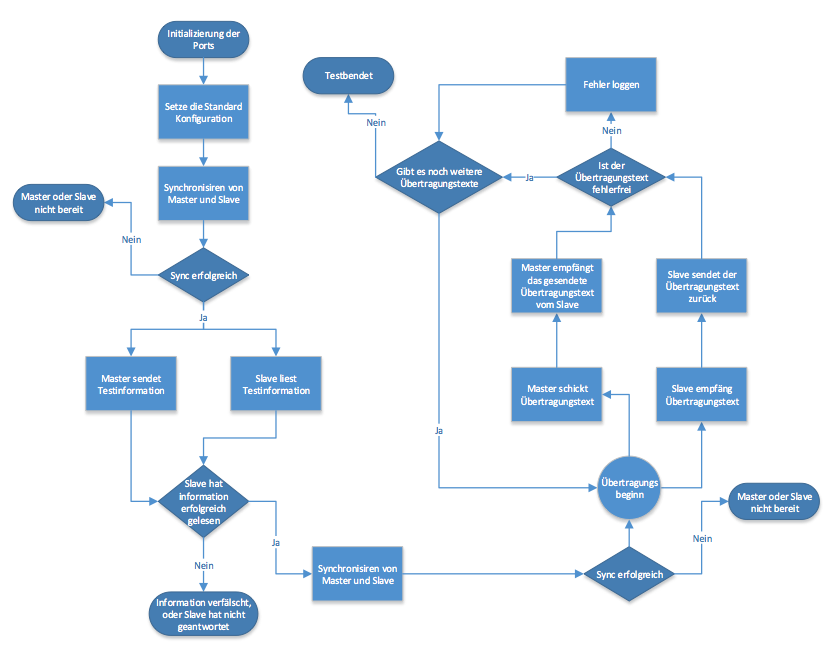
\includegraphics[scale=0.5]{MasterSlave.png}
  		  \caption{Ablauf des Master-Slave Test}
     \label{MasterSlaveDiagramm}
  \end{center}
\end{figure}


%\newpage


Die Synchronisation der beiden COM Ports geschieht indem der Master ein Fluchtzeichen (Escape-Sequenzen) sendet  und der Slave antwortet. Der Master sendet ein "`ESC"' (ASCII 0x1B) und wartet auf die Antwort vom Slave, was in Form von einem "`ACK"' (ASCII 0x06) gesendet wird. Wenn beide COM Ports synchron sind, schickt der Master dem Slave eine "`Kopfzeile"'. In dieser Kopfzeile steht die Nummer der zu übertragenden Zeile, sowie die Anzahl der zu übertragenen Bytes, jeweils mit einer Breite von drei Zeichen. Die Kopfzeile hat folgendes Format:

\begin{center}
<Zeilennummer-Anzahl\_An\_Bytes>\\

<001-010>
\end{center}

Die Kopfzeile ist nötig, damit der Slave weiß, wie viele Zeichen im Übertragungstext, bei der nächsten Übertragung, ankommen werden, damit die richtige Anzahl an Bytes aus dem Puffer gelesen werden kann. Nachdem die Kopfzeile empfangen worden ist, und der Slave seinen Inhalt interpretieren kann, wird ein "`ACK"' gesendet, damit der Master weiß, dass die Kopfzeile erfolgreich übertragen worden ist. Wenn der Master das "`ACK"' aus seinen Puffer liest, schickt er die erste Information an den Slave zurück. Diese Information ist die gewünschte Testeinstellung.

\begin{center}
baudrate;parität;stopbits;datenbits;protokoll\\
9600;1;2;8;2
\end{center}

\newpage

Der Slave liest die ankommende Information und schickt ein "`ACK"' zurück. Danach wird die Information auf valide Werte überprüft und die Einstellungen werden gespeichert. In diesem Moment sind beide Schnittstellen synchron und bereit den Testvorgang mit den gewünschten Testeinstellungen zu starten. In beiden Schnittstellen werden die gewünschten Einstellungen gesetzt, und die Schnittstellen versuchen sich erneut zu synchronisieren. Ist die Synchronisation erfolgreich, schickt der Master erneut eine Kopfzeile an den Slave und danach den Übertragungstext. Der Slave antwortet auf die Kopfzeile beim erfolgreichen Empfangen mit einem "`ACK"' und beim Empfang vom Übertragungstext wird dieser zurück geschickt. Nachdem der Master den Übertragungstext versendet, wartet er auf die Antwort des Slaves in Form vom versendeten Text. Der Master liest den empfangenen Text aus seinem Puffer und vergleicht es mit dem versendeten Text. Werden keine Fehler festgestellt, wird der Vorgang wiederholt bis das Ende der Übertragung erreicht ist.


%****************************************************************************************
\newpage
%****************************************************************************************


\section{Klasse IniFileHandler}\label{IniFileHandler}
\paragraph{}
Die Klasse \textit{IniFileHandler} behandelt das Lesen und Speichern von Testeinstellungen in einer Datei, einer so genannten Testkonfigurationsdatei. Das Format dieser Datei basiert auf der von Windows vorgegebenen Initialisierungsdateien (.ini, INI-Datei). Mit Hilfe der Methoden \textit{WritePrivateProfileString}\footnote{http://msdn.microsoft.com/en-us/library/windows/desktop/ms725501(v=vs.85).aspx; 22.09.2013} und \textit{GetPrivateProfileString}\footnote{http://msdn.microsoft.com/en-us/library/windows/desktop/ms724353(v=vs.85).aspx; 22.09.2013} können jeweils die Testparameter geschrieben und gelesen werden. Das Format einer INI-Datei ist folgendermaßen aufgebaut:\\

\hspace*{20mm}\textit{[Sektion]}    \\
\hspace*{20mm}\textit{;Kommentar}    \\
\hspace*{20mm}\textit{Variable=Wert}\\

In Kapitel \ref{chp:bedienungsanleitung} werde genauer die Parameter und die Werte für eine Datei erläutert. Die Klasse ist in drei Arten von Methoden getrennt, diese sind Lese-, Schreib- und Übersetzermethoden.\\

\subsection{Übersetzer}
\paragraph{}
Die Übersetzermethoden bekommen einen Parameter, der entweder geschrieben oder im Programm gespeichert wird. In beiden Fällen muss der Parameter auf Gültigkeit geprüft werden. Wird der Parameter in einer INI-Datei geschrieben, muss er in manchen Fällen, wie zum Beispiel bei der Baudrate, zuerst von einer Zahl auf einen String umgewandelt werden. Wird die Baudrate gelesen, muss dieser String auf eine Zahl umgewandelt werden und geprüft werden, ob der gelesene/umgewandelte Wert ein gültiger Wert ist. Dieser Vorgang gilt für alle anderen Parameter auch.



\subsection{Schreiben}
\paragraph{}
Durch den Aufruf der Methode \textit{WritePrivateProfileString} mit folgenden Parameter wird die Baudrate in eine Datei gespeichert:\\

\begin{lstlisting}
	WritePrivateProfileString(ComPort,"Baudrate","9600", Dateipfad);
\end{lstlisting}

Die Variable \textit{Dateipfad} spezifiziert die Zieldatei in der die Schlüssel/Variable \textit{Baudrate} geschrieben werden soll. Der Wert für den Eintrag ist \textit{9600}. Der Eingabeparameter \textit{ComPort} ist die Bezeichnung für einen COM Port und gibt an in welcher Sektion die Variable \textit{Baudrate} geschrieben werden soll. Der Eintrag für den Aufruf dieser Methode lautet:\\

\hspace*{20mm}\textit{[COM2]}    \\
\hspace*{20mm}\textit{;Das ist die Baudrate}    \\
\hspace*{20mm}\textit{Baudrate=9600}\\

Auf diese Weise werden alle Testeigenschaften in einer INI-Datei gespeichert. Durch die Trennung von Sektionen werden die Parameter für verschiedene COM Ports bei einem neuen Eintrag nicht überschrieben.


\subsection{Lesen}
\paragraph{}
Will der Benutzer Werte, beziehungsweise die Baudrate, aus einer INI-Datei lesen, muss er die Methode \textit{GetPrivateProfileString} mit folgenden Parametern aufrufen:\\

\begin{lstlisting}
	GetPrivateProfileString(ComPort, "Baudrate", NULL,
                        Puffer, GrößeDesPuffers, Dateipfad);
\end{lstlisting}

Die bekannten Parameter sind die gleichen wie bei der Schreibmethode. \textit{Puffer} ist eine Variable, in der der gelesene Wert geschrieben wird und \textit{GrößeDesBuffers} gibt die Größe des Puffers an. So wird der String \textit{9600} in die Variable \textit{Puffer} geschrieben. Durch Aufruf der entsprechenden Übersetzermethode, wird die gelesene Baudrate in eine Zahl umgewandelt und im Programm gespeichert.


%****************************************************************************************
\newpage
%****************************************************************************************

\section{Klasse Tools}
\paragraph{}
Die Klasse \textit{Tools} ist eine Sammlung von verschiedenen Hilfsmethoden, die in den anderen Klassen aufgerufen werden.

  
\subsection{String Methoden}
\paragraph{}
In den anderen Klassen ist es immer wieder nötig Variablen in Strings umzuwandeln. Die Methode \textit{convertToString} konvertiert ganze Zahlen, Multibyte Zeichenketten und Zeiger auf Zeichenketten zu einem String. Der Eingabeparameter der Funktion wird in einen \textit{stringstream} geschrieben und dieser Stream wird als String zurückgegeben.\\

Eine weitere Methode heißt \textit{printTime}, diese Methode fragt die Uhrzeit im System ab und schreibt diese in einen String, der zurück gegeben wird. Die Methode \textit{delSpaces} löscht alle Leerzeichen in das an die Methode übergebene String. 

\begin{lstlisting}
	s.erase(remove_if(s.begin(), s.end(), isspace),s.end());
\end{lstlisting}

Der Löschvorgang wird mit Hilfe von der String-Klassenmethode \textit{erase} und der \textit{Template Class} \textit{remove\_if} durchgeführt. Die Anfang- und Enditeratoren des Strings werden an die \textit{Templa Class} gegeben somit wird das Zeichen markiert welches gelöscht werden soll. Die Zeichen sind alle Leerzeichenmöglichkeiten (Tabs, CarriageReturn, NewLine, etc.) zu verstehen, diese werden durch die Funktion \textit{isspace} abgefragt und von der \textit{erase} Methode gelöscht.\\

Die letzte Methode teilt die durch Leerzeichen übergebene Zeichenkette in einzelnen Strings und schreibt diese in einen Vektor vom Typ String. Diese Methode wird angewendet um die, über die Kommandozeile eingegebenen Parameter zu erkennen und einzeln auswerten zu können. Die letzte Stringmethode wird für den Übertragungstext benutzt. Wenn ein Übertragungstext so genannte Fluchtzeichen beinhalten soll, werden diese als Hexadezimalwerte eingegeben und in dieser Methode durch ein Zeichen ersetzt.

\subsection{Weitere Methoden}
\paragraph{}
Eine andere Art von Methoden in dieser Klasse ist die \textit{printErrorVector} Methode. Diese Methode gibt die Ergebnisse der Tests aus, jeweils über die GUI als Fenster oder in der Logdatei. Die Methode \textit{errorCodeParser} bekommt als Eingabeparameter ein Exitcode eines Funktionsaufrufes und gibt die Erklärung dieses Exitcodes als String zurück. Die \textit{wait} Methode bekommt eine Zahl als Eingabeparameter. Diese Zahl dient als Multiplikator mit dem die Zehn Millisekunden multipliziert werden, das Ergebnis ist die zu wartende Zeit. Die Methode wird bei der Synchronisierung von einen Master und einen Slave benutzt. Die letzte Methode in der Klasse \textit{Tools} zeigt dem Benutzer einen Hilfetext an, wenn falsche Eingabeparameter in der Kommandozeile eingegeben worden sind.



%****************************************************************************************
\newpage
%****************************************************************************************


\section{Klasse TransferFileHandler}
\paragraph{}
Die Klasse \textit{TransferFileHandler} behandelt die Dateien die in einer Übertragung gesendet werden sollen. Die Klasse öffnet, liest und schließt die Datei.

\subsection{Aufbau}
\paragraph{}
Die Klasse öffnet mittels der Methode \textit{openFile} eine Datei die als Eingabeparameter angegeben worden ist. Eine Variable vom Typ \textit{ifstream} (input file stream) wird deklariert. Durch die Methode \textit{open} wird der Pfad der Datei angegeben und die Methode versucht diese Datei zu öffnen. Falls die Datei nicht geöffnet werden konnte, wird der Benutzer benachrichtigt. Ist die Datei erfolgreich geöffnet worden, wird jede Zeile in der Datei bis zum Ende gelesen und in einem Vektor gespeichert. Danach wird die Datei geschlossen.\\


%****************************************************************************************
\section{Klasse Logger}\label{LoggerClass}
\paragraph{}
Die Klasse \textit{Logger} erzeugt auf Wunsch des Benutzers eine Logdatei, worin alle Testereignisse geschrieben werden. Wird ein Objekt von der Klasse \textit{Logger} erzeugt, wird als erstes eine Datei im "`\%temp\%"' Ordner angelegt und der Puffer des Objekts \textit{clog} (output stream) auf die Logdatei umgeleitet. Ein Beispiel einer Logdatei, bitte siehe Anhang ~\ref{LogDatei}.\\



%****************************************************************************************
\section{Header Constants}
\paragraph{}
In die Headerdatei \textit{Constants} werden alle Konstanten für das Programm deklariert. Unter anderem sind hier die Werte für:

\begin{itemize}
\item Programmversion
\item ID der GUI-Elemente
\item Errorcodes
\item Baudraten
\item TestStruct (siehe \ref{TestStruct})
\end{itemize}

deklariert.
\chapter{Testbeschreibung}\label{chp:Testbeschreibung}
\paragraph{}
Als letzter Schritt für die Beendigung der Entwicklung des Testprogrammes müssen Test für die Funktionseinheiten und die Benutzerschnittstelle durchgeführt werden. 


\section{Benutzerschnittstelle}
\paragraph{}
In den Tests für die Benutzerschnittstellen müssen alle Parameter getestet werden, in die der Benutzer einen Fehler eingeben kann. Im Testprogramm gibt es einen Abschnitt wo alle Parameter überprüft werden. Folgende Testfälle (siehe Tabelle) müssen von diesem Programmabschnitt abgefangen werden und dem Benutzer gemeldet werden, welche Eingaben fehlerhaft waren. Diese Fehleingaben werden mit einer passende Fehlermeldung dem Benutzer ausgegeben. Folgende Teststrategien werden ausgeübt:

\begin{tabular}{lll}

&\textbf{Positivtest:} &erwartete Eingabe für den jeweiligen Parameter (bei einer Zahl wird eine gültiger\\
& & numerischer Wert eingegeben)\\

&\textbf{Negativtest:} &unerwartete Eingabe für den jeweiligen Parameter (bei einer Zahl wird ein Text\\
& & eingegeben)\\

&\textbf{Grenzwerttest:} &gültige und ungültige Grenzwerte\\
\end{tabular}

Für die Dokumentation der Tests werden die Positivtests nicht berücksichtigt. 


\subsection{INI-Datei}
\paragraph{}
In einer INI-Datei müssen alle gelesenen Parameter auf plausible Werte überprüft werden. Eine Liste mit den Bedeutungen der Errorcodes ist im Anhang \ref{Errorcodes} nach zu schlagen.
\begin{longtable}{||l|p{3cm}|p{5cm}|c||}
 
%  Als Kopfzeile & der anderen Seiten & wird dies gesetzt &\\ \hline
%  \endhead
%  Die Fu"szeilen & f"ur & alle Seiten & \\ \hline\hline
% \endfoot
%  Nur die letzte & Fu"szeile ist etwas & BESONDERES &\\ \hline\hline
%  \endlastfoot


\hline
Testfall & Fehler & Kommentar & Errorcode \\ \hline\hline
\endfirsthead
\hline
Testfall & Fehler & Kommentar & Errorcode \\ \hline\hline
\endhead

COM0   & falscher COM Port & kein gültiger Wert, Datei wird als Leer interpretiert & -12\\ \hline
COM1   & falscher COM Port & nicht im System vorhanden                             & -6 \\ \hline
COM256 & falscher COM Port & nicht im System vorhanden                             & -6 \\ \hline
COM257 & falscher COM Port & kein gültiger Wert, Datei wird als Leer interpretiert & -12\\ \hline\hline

baudrate=Min-Max     & falscher Parameter        & MIN-MAX                      & -17 \\ \hline
baudrate=-MAX        & unvollständiger Parameter & fehlt eine minimale Baudrate & -17 \\ \hline
baudrate=MIN-        & unvollständiger Parameter & fehlt eine maximale Baudrate & -17 \\ \hline
baudrate=-9600-115200& negative Baudrate         & ungültige Eingabe wird nicht interpretiert &  -15\\ \hline

parity=Min-Max & falscher Parameter & MIN-MAX         & -9\\ \hline
parity=1       & falscher Parameter & nur Text & -9\\ \hline
parity=ODD     & falscher Parameter & odd, even, none & -9\\ \hline\hline

databits=6    & falscher Parameter & 7, 8       & -9\\ \hline
databits=9    & falscher Parameter & 7, 8       & -9\\ \hline
databits=text & falscher Parameter & nur Zahlen & -9\\ \hline\hline

protocol=0    & nur Text             & none, hardware, XON/XOFF & -9\\ \hline
protocol=NONE & falscher Parameter & none, hardware, XON/XOFF & -9\\ \hline\hline

stopbits=text & nur Zahlen           & 1, 2 & -9\\ \hline
stopbits=0    & falscher Parameter & 1, 2 & -9\\ \hline
stopbits=3    & falscher Parameter & 1, 2 & -9\\ \hline\hline

transfertextmode=sometext & falscher Parameter & default, text, file   & -9\\ \hline
transfertextmode=default  & & &\\
transfertext=teststring   & unnötiger Parameter  & wird nicht betrachtet & 0 \\ \hline

transfertextmode=file & & &\\
transfertext                  & nicht definiert      & Dateipfad muss angegeben werden     & -9\\ \cline{2-4}
transfertext=                 & leerer Parameter     & Parameter muss angegeben werden     & -9\\ \cline{2-4}
transfertext=C:\textbackslash & ungültiger Dateipfad & gültiger Pfad muss angegeben werden & -13\\ \hline\hline

transfertextmode=text & & &\\
transfertext                  & nicht definiert      & Übertragungstext muss angegeben werden & -9\\ \cline{2-4}
transfertext=                 & leerer Parameter     & Parameter muss angegeben werden        & -9\\ \hline\hline

logger=keine & falscher Parameter & true, false & -9\\ \hline
logger=123   & falscher Parameter & true, false & -9\\ \hline\hline

stoponfirsterror=nein & falscher Parameter & true, false & -9\\ \hline
stoponfirsterror=321  & falscher Parameter & true, false & -9\\ \hline\hline

repeater=-1   & falscher Parameter & nur Zahlen $\geq$ 0 & -9\\ \hline
repeater=text & falscher Parameter & nur Zahlen $\geq$ 0 & -9\\ \hline\hline

\end{longtable}


Bei einer Testdatei mit mehreren Sektionen, werden zuerst alle Eingaben gelesen und geprüft. Wird ein Fehler gefunden, wird dieser dem Benutzer gemeldet. Sind ungültige Sektionen wie [COM0] oder [COM257] in der Testdatei eingetragen, werden diese vom Testprogramm nicht betrachtet. Alle anderen gültigen Eingaben werden geprüft und getestet.


\subsection{Kommandozeile}
\paragraph{}
In der Kommandozeile kann der Benutzer eine vollständige Testdatei angeben oder eine Testdatei wo die Sektion als [COM] definiert ist, plus die Angabe welcher Port getestet werden soll.

\hspace*{10mm}\textit{SerialPortTester.exe C:\textbackslash Testdateien\textbackslash Testdatei1.ini}\\
\hspace*{10mm}\textit{SerialPortTester.exe C:\textbackslash Testdateien\textbackslash Testdatei2.ini /COM1}\\

\begin{longtable}{||l|p{3cm}|p{5cm}|c||}
\hline
Testfall & Fehler & Kommentar & Errorcode \\ \hline\hline
\endfirsthead
\hline
Testfall & Fehler & Kommentar & Errorcode \\ \hline\hline
\endhead

C:\textbackslash Testdateien & falscher Dateipfad & Dateipfad gibt keine Datei an & -12\\ \hline
C:\textbackslash Testdateien\textbackslash Datei & falscher Dateipfad & Dateipfad gibt keine gültige Testdatei an & -12\\ \hline

C:\textbackslash Testdatei.ini /com1 & falscher COM Port & Portbezeichnung ungültig, muss COM1 sein & -1\\ \hline
C:\textbackslash Testdatei.ini /COM0 & falscher COM Port & Portname ungültig & -1\\ \hline
C:\textbackslash Testdatei.ini COM1 & falscher Parameter & Parameter muss mit / beginnen & -1\\ \hline

C:\textbackslash Testdatei.ini /COM1 /COM2& falscher Parameter & zu viele Parameter & -1\\ \hline
/COM0 & falscher Parameter & Dateipfad fehlt &-1 \\ \hline

\end{longtable}


\subsection{Benutzeroberfläche}
\paragraph{}
In der Benutzeroberfläche werden nur gültige Parameter angeboten, außer die Baudraten, der Wiederholungszähler (Repeater), die Übertragungsdatei und der Übertragungstext. Die Baudraten werden für jeden COM Port vom System abgefragt. Durch die Tests wurde festgestellt, dass manche Baudraten angeboten werden, die nicht wirklich unterstützt werden. Der Benutzer kann im Fehlerfall, mit Hilfe der Kommandozeile und den Befehl \textit{mode} sicherstellen, dass die Baudrate tatsächlich nicht unterstützt wird. Bei den anderen Parametern werden Fehler erkannt, da die Überprüfung für die GUI oder Testdatei die gleiche ist.



\section{Funktionseinheiten}
\paragraph{}
Die Funktionstests basieren auf den Funktionen des Testprogrammes. Die verschiedenen Einstellungsmöglichkeiten werden getestet. Durch die Ausführlichkeit des Tests werden nur die durchgefallenen Tests erläutert. Laut den  Testergebnissen gibt es keine Einschränkungen in den Testmodi (Automatic, Wobble und Fixed) und in den Transfermodi \textit{Shorted} und \textit{Double}. Wird der Transfermodus \textit{Master-Slave} in einem System getestet, wurden keine Probleme erkannt. Wird die gleiche Einstellung in zwei verschiedenen Systemen ausgeführt, kommt es öfters zu Synchronisierungsproblemen nach dem ersten Testschritt\footnote{Unter Testschritt ist zu verstehen, dass ein Test aus mehreren Schritten besteht. Für jede mögliche Testkonfiguration wird ein Testschritt definiert. Wird für ein \textit{Fixed-Shorted} Test der Wiederholzähler auf Zehn gesetzt, besteht dieser Test aus Zehn Testschritten}. Wenn beide Schnittstellen im ersten Testschritt sich erfolgreich synchronisieren und den ersten Testschritt erfolgreich abschließen, müssen sich für einen neuen Testschritt nochmal synchronisieren. Bei diesen Vorgang kommt es zu einem Fehler und beide Schnittstellen erkennen sich nicht.
\chapter{Bedienungsanleitung}\label{chp:bedienungsanleitung}
\paragraph{}
Das Testprogramm kann über die Kommandozeile oder direkt über die Benutzeroberfläche bedient werden. Je nach Testmodus muss der Benutzer folgende Parameter angeben, um erfolgreich einen Test zu starten:


In beiden Fällen  je nach Testmodus, 
\\
\begin{tabular}{llll}
\\ &\textbf{Parameter} & &\textbf{GUI Element}
\\ &COM Port &: &Main Port
\\ &Baudrate &: &Baud rate
\\ &Test Modus &: &Test Mode
\\ &Übertragungsmodus &: &Transfer
\\ &Slave Port &: &Slave Port
\\ &Maximale Baudrate &: &MAX baud rate
\\ &Parität &: &Parity
\\ &Übertragungsprotokoll &: &Protocol
\\ &Stopbits &: &Stopbits
\\ &Datenbits &: &Databits
\\ &Übertragungsdatei &: &Load file to be transfered
\\ &Übertragungstext &: &Send text
\\ &Logger &: &Logger
\\ &Wiederholungszähler &: &Repeater
\\ &Beim ersten Fehler anhalten &: &Stop on 1. error
\\ &Start &: &Start
\\ &Schließen &: &Close
\\ &Speichern &: &Save
\\ &Testdatei laden &: &Load test file
\\ &Hilfe &: &Help
\\ &Stop &: &Stop
\end{tabular}

Eine vollständige Liste der Errorcodes, die das Programm erzeugen kann,  ist im Anhang \ref{Errorcodes}.

\section{Bedienung über die GUI}
\paragraph{}
Mit der GUI kann der Benutzer einen Test starten, mit einer Eingabe von Parametern oder durch das Laden einer Testdatei. Der Benutzer kann auch eine Testdatei erstellen, in dem er die Parameter in der GUI einstellt und diese speichert.

\section{Bedienung über die Kommandozeile}
\paragraph{}
Über die Kommandozeile kann der Benutzer eine Testdatei und den zu testende Port angeben. Wenn keine Parameter angegeben worden sind, wird die GUI gestartet. Um eine Testdatei zu laden muss folgender Programmaufruf erfolgen:
\begin{center}
\textit{SerialPortTester.exe Dateipfad\textbackslash Testdatei.ini}
\end{center}

Um einen speziellen Port zu testen, muss dieser Port noch dazu angegeben werden. Bitte beachten, dass die Testdatei nur die Konfiguration für einen Port haben darf, die "`Sektion"' muss "`[COM]"' heißen. Um den COM Port COMx zu testen, muss der Programmaufruf folgendermaßen gestaltet sein:

\begin{center}
\textit{SerialPortTester.exe Dateipfad\textbackslash Testdatei.ini /COM1}
\end{center}

Um den Testvorgang zu stoppen, kann der Benutzer die ESC-Taste drücken. Es kann zu einer Verzögerung beim Beenden des Programmes kommen (besonderes bei niedrigen Baudraten oder langen Übertragungstexten), da die angefangene Übertragung nicht unterbrochen wird.


\section{Testmodus}

\subsection{Automatic}
\paragraph{}
Der Automatic Test ist ein vordefinierter Testfall. Für diesen Test muss der Benutzer nur den Übertragungsmodus und den zu testenden Port angeben. Der Test wird immer mit folgenden Parametern gestartet.
\\
\begin{tabular}{llll}
\\ &\textbf{Parameter} & &\textbf{Wert}
\\ &Main Port &: &Vom Benutzer wählbar
\\ &Baud rate &: &9600
\\ &Test Mode &: &Automatic
\\ &Transfer &: &Vom Benutzer wählbar
\\ &Slave Port &: &Wenn nötig, vom Benutzer wählbar
\\ &Parity &: &Odd
\\ &Protocol &: &Hardware
\\ &Stopbits &: &1
\\ &Databits &: &8
\\ &Send text &: &Default, fest kodiert
\\ &Logger &: &Ja
\\ &Repeater &: &Unendlich
\end{tabular}

Der Test wird so lange wiederholt bis der Benutzer den Test stoppt oder wenn die Eigenschaft \textit{stop on first error} gesetzt ist und ein Fehler erkannt wird.



\subsection{Wobble}
\paragraph{}
In einem Wobble Test kann der Benutzer alle Parameter einstellen. Die wichtigsten Parametern sind die minimale und maximale Baudrate. Diese Werte geben die Unter- und Obergrenze der Baudraten an. Alle Standard einstellbaren Baudraten werden für einen Test eingestellt. Es ist möglich zwischen drei verschiedenen Paritätseinstellungen (ungeraden, gerade und keine Parität) zu wobbeln. Diese Option ist nur über eine Testdatei einstellbar.


\subsection{Fixed}
\paragraph{}
Im Fixed Test muss der Benutzer alle Parameter einstellen. In diesem Testverlauf werden sich die Parameter nicht ändern und der gleiche Test wird so oft wiederholt wie in der Option "`Repeater"'.



\section{Übertragungsmodus}
\paragraph{}
Jeder Testmodus kann in vier Übertragungsmodus eingestellt werden, die den Testablauf bestimmen. Die Einstellungen für einen Übertragungsmodus sind abhängig von dem eingestellten Testmodus.

%Für ein "`Shorted"' Test muss an dem ausgewählten COM Port ein Kurzschlussstecker angeschlossen werden. Bei einem "`Double"' oder "`Master - Slave"' Test müssen die beteiligten Schnittstellen mit einem Null-Modemkabel verbunden werden.

\subsection{Shorted}
\paragraph{}
Im Shorted Modus muss an der angegebenen Schnittstelle ein Kurzschlussstecker angeschlossen werden. Hier ist der Port, Master und Slave gleichseitig. Der Port schickt und empfängt die Daten sofort.


\subsection{Double}
\paragraph{}
Hier werden zwei COM Ports in einem System getestet. Mittels eines Null-Modem-Kabel wird Port1 an Port2 angeschlossen. Port1 sendet die Übertragungsinformation und Port2 empfängt diese.


\subsection{Master}
\paragraph{}
Der Master Modus verlangt zwei verschiedene Systeme. Im System1 schickt der Master Daten und wartet auf eine Antwort. Der Master kennt seinen Slave nicht. System1 und System2 werden durch ein Null-Modem-Kabel verbunden. Der Master macht die Fehlerauswertung, so lange keine Lese- oder Schreibfehler im Slave geschehen sind.


\subsection{Slave}
\paragraph{}
Der Slave im System2 wartet auf den Eingang der Daten von System1. Der Slave kennt sein Master nicht, er empfängt Daten und schickt die gleichen Daten zurück, damit der Master die Fehlerauswertung durchführen kann. Im Slave Modus müssen nur folgende Parameter eingestellt werden:

\begin{itemize}
\item COM Port
\item Bei einem "`Double"' Test die minimale und maximale Baudrate
\item Logger
\item Repeater (gleicher Wert wie der Master)
\item Textübertragungsmodus
\item Übertragungstext oder Übertragungsdatei
\end{itemize}


\section{Schnittstelleneigenschaften}

\paragraph{Baudrate} Die Baudrate mit der getestet werden soll
\paragraph{Parity} Hier kann der Benutzer zwischen gerade, ungerade oder keine Parität auswählen
\paragraph{Protocol} Der Benutzer ist in der Lage das Übertragungsprotokoll zu bestimmen. Zur Auswahl steht Xon/Xoff, Hardware oder kein Protokoll
\paragraph{Stopbits} Mit diesem Parameter werden die Stopbits eingestellt, entweder 1 oder 2 Stopbits
\paragraph{Databits} Hier wird bestimmt, wie viele Bits ein Zeichen hat, 7 oder 8 Bits pro Zeichen

\section{Sendedaten}
\paragraph{}
Durch klicken der Schaltfläche "`Load file to send"' kann der Benutzer eine Datei auswählen, diese wird dann beim Testen geöffnet und Zeilenweise verschickt. Ist eine Zeile in der Übertragungsdatei länger als 100 Zeichen, werden nur die ersten 100 Zeichen betrachtet. Möchte der Benutzer einen spezifischen Text senden, muss er diesen unter "`Send text"' eingeben und "`Load text to send"' klicken. In einer Testdatei darf der Übertragungstext nicht länger als 100 Zeichen lang sein. Wenn keiner dieser beiden Möglichkeiten benutzt wird, wird ein im Programm fest kodierter Text übertragen.

\section{Logger}
\paragraph{}
Wenn die Checkbox ausgewählt ist, wird eine Textdatei im "`\%temp\%"' Verzeichnis angelegt und alle Meldungen werden dort mitgeloggt. Die Datei hat immer den Namen des Ports, der getestet wird. Bei schreibgeschützten Medien, wie im Fall von Windows PE , darf diese Option nicht gewählt werden.


\section{Wiederholungszähler}
\paragraph{}
Der Wiederholzähler gibt an, wie oft ein Testschritt wiederholt werden soll. Unter Testschritt ist zu verstehen, jeder Schreibe- und Lesevorgang mit verschiedenen einstellbaren Parametern.


\section{Beim ersten Fehler anhalten}
\paragraph{}
Diese Option gilt für die Fehlersuche. Wenn diese Option gesetzt ist, hält das Testprogramm beim ersten erkannten Fehler an. So kann der Tester nach Fehler suchen. Wenn diese Option nicht gesetzt ist, werden die Fehler am Ende des Testvorgangs gemeldet oder geloggt. So kann eine Fehlerstatistik erzeugt werden.


\section{Buttons}
\paragraph{Start} Beginnt einen Test mit den eingegeben Parametern
\paragraph{Close} Beendet das Test Tool
\paragraph{Save} Speichert die ausgewählten Einstellungen in einer Testdatei
\paragraph{Load test file} Lädt eine vom Benutzer ausgewählte Testdatei
\paragraph{Help} Zeigt die Hilfe zum Programm
\paragraph{Stop} Stoppt den Testvorgang. Es kann zu einer Verzögerung beim Beenden des Programmes kommen (besonderes bei niedrigen Baudraten oder langen Übertragungstexte), da die angefangene Übertragung nicht unterbrochen wird



\section{Testdatei}
\paragraph{}
In einer Testdatei wird die Testkonfiguration gespeichert. Eine Testdatei kann manuell oder mit Hilfe der GUI erzeugt werden. Die Testdatei ist wie eine Datei aus der Registrierungsdatenbank (Windows Registry)aufgebaut. In "`[ ]"' wird der Port angegeben und darunter die jeweilige Testparameter. Für ein Beispiel siehe bitte Anhang \ref{TestDatei}.


\section{Einstellbare Werte}
\paragraph{}
Die Einstellparameter können folgende Werte in der GUI oder Testdatei zugewiesen bekommen:
\paragraph{Main/Master und Slave Port} im System vorhandene COM Ports. Diese werden für den Benutzer in der GUI aufgelistet.
\paragraph{Baudrate} Für den ausgewählten COM Port einstellbare Baudraten
\paragraph{Test Mode} automatic, wobble, fixed
\paragraph{Transfer Mode} shorted, double, master, slave
\paragraph{Parity} none, odd, even
\paragraph{Protocol} XON/XOFF, hardware, none
\paragraph{Stopbits} 1, 2
\paragraph{Databits} 7, 8
\paragraph{File to send} Pfad zu einer Testdatei. Wenn eine Zeile länger als 100 Zeichen ist, werden nur die ersten 100 Zeichen Übertragen
\paragraph{Text to send} Vom Benutzer auswählbarer String der übertragen wird. Wenn eine Zeile länger als 100 Zeichen ist, werden nur die ersten 100 Zeichen übertragen
\paragraph{Logger} Gibt an ob eine Log-Datei angelegt wird oder keine
\paragraph{Repeater} Anzahl der Testwiederholungen


\section{Einfaches Beispiel}
\paragraph{}
Ein Benutzer will zum Beispiel den Port COM1 testen. Dieser soll an den COM2 Port die Wörter "`Hallo Welt"' schicken. Als Baudrate ist 9600 vorgegeben, mit einer geraden Parität, Xon/Xoff Protokoll, sieben Datenbits und zwei Stopbits. Der Test soll fünfmal wiederholt werden und eine Log-Datei soll geschrieben werden.

\paragraph{}
Als erstes muss der Benutzer unter \textit{Main Port} "`COM1"' auswählen. Danach werden die möglichen Baudraten in \textit{Baud rate} aufgelistet. Dort muss der Benutzer 9600 wählen. Da nur eine bestimmte Konfiguration gegeben ist, ohne Variablen, wird auf "`Fixed"' unter \textit{Test Mode} geklickt und als Übertragungsmodus "`Double"' ausgewählt. Unter \textit{Parity} wird "`Even"', \textit{Protocol} wird "`XON/XOFF"', \textit{Stopbits} wird "`2"' und \textit{Databits} wird "`7"' ausgewählt.\\

\begin{figure}[h]
  \begin{center}		%width=\linewidth
    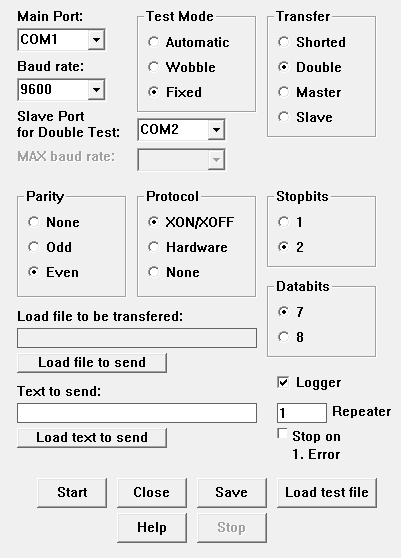
\includegraphics[scale=0.4]{Beispiel1}
  		  \caption{Beispiel der Testeinstellungen}
     \label{Beispielbild 1}
  \end{center}
\end{figure}

\newpage

\paragraph{}
Unter \textit{Send text} soll der Benutzer "`Hallo Welt"' schreiben. Will der Benutzer Escape-Sequenzen schicken, müssen diese als Hexadezimal Werte angegeben werden (zum Beispiel \textbackslash0a oder \textbackslash0d). Danach wird auf \textit{Load text to send} geklickt. Ein Pop-Up Fenster meldet, dass der Text geladen worden ist. Damit der Test fünfmal wiederholt wird, muss im \textit{Repeater} eine fünf anstatt der eins eingetragen werden. Danach ist die GUI konfiguriert und der Benutzer kann auf \textit{Start} klicken.\\

\begin{figure}[h]
  \begin{center}
    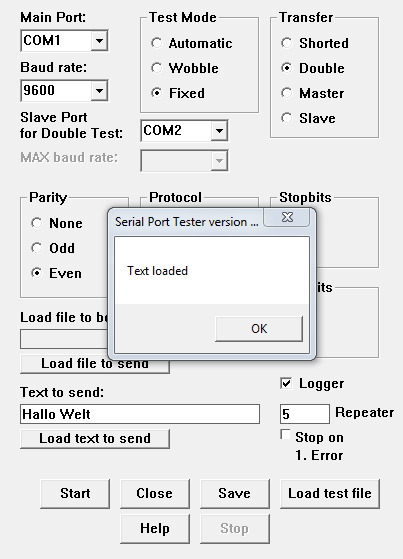
\includegraphics[scale=0.4]{Beispiel2}
  		  \caption{Beispiel laden eines Textes}
     \label{Beispielbild 2}
  \end{center}
\end{figure}

\paragraph{}
Durch ein Pop-Up Fenster wird dem Benutzer gemeldet, wenn der Test abgeschlossen ist. Um eine Evaluation des Tests machen zu können muss die Log-Datei ausgewertet werden.


\chapter{Zusammenfassung und Ausblick}\label{chp:zusammenfassung}
%Lehnen Sie sich zurück von Ihrem Terminal und versuchen ein wenig Abstand zu den vielen Detail-Problemen Ihrer Diplomarbeit zu gewinnen:
%Was war wirklich wichtig bei der Arbeit? 
%Wie sieht das Ergebnis aus?
%Wie schätzen Sie das Ergebnis ein?
%Gab es Randbedingungen, Ereignisse, die die Arbeit wesentlich beeinflußt haben?
%Gibt es noch offene Probleme?
%Wie könnten diese vermutlich gelöst werden?\\\\


\paragraph{}


Durch die Verwendung der Windows API konnte ich meine Kenntnisse und das Verständnis für das Windows Betriebssystem erweitern. Leider war es schwer aktuelle Quellen und Literatur für die Entwicklung des Programms "`SerialPortTester"' zu finden. Da die Windows API heutzutage kaum noch eine Verwendung findet und der Trend in Richtung des .NET Frameworks geht, kann nur auf die Windows API als Referenz zurückgegriffen werden. Durch das selbständige Entwickeln dieser Bachelorarbeit konnte ich viel Erfahrung in der Planung und Entwicklung eines Projektes sammeln. Ebenso konnte ich meine Programmierkenntnisse erweitern. \\
 

Durch die Verkürzung meiner Bearbeitungszeit der Bachelorarbeit konnte ich einen Punkt der Anforderungsliste nicht fertigstellen. Im \textit{Master-Slave} Test (zwei getrennte Systeme) tritt zurzeit noch ein Fehler auf, wenn mehr als eine Wiederholung dieses Testschrittes durchgeführt werden soll. Dabei werden die Schnittstellen im folgenden Testschritt nicht mehr synchronisiert. Ein weiterer Punkt ist eine bessere Lösung hinsichtlich der Wartezeit-Strategie (der Slave muss 3 Sekunden nach dem Start des Mastertest gestartet werden) für die Initialisierung des \textit{Master-Slave} Tests zu entwickeln.\\

Das Programm könnte in Hinsicht der Einstellungsparameter Stopbits, Datenbits und die Parität erweitert werden. Es gibt noch die Möglichkeit 1.5 Stopbits einzustellen, aber dieses wird nur bei niedrigeren Anzahl als 7 und 8 Datenbits unterstützt. Im Fall von der Parität könnten die Eigenschaften \textit{Markierung} und \textit{Leerzeichen} noch hinzugefügt werden.

\listoffigures %Abbildungsverzeichnis
%\lstlistoflistings
%--------------------------------------------------------------%
% Anhang
%--------------------------------------------------------------%

\begin{appendix}
	%%
%% Beuth Hochschule für Technik --  Abschlussarbeit
%%
%% Anhang
%%
%%%%%%%%%%%%%%%%%%%%%%%%%%%%%%%%%%%%%%%%%%%%%%%%%%%%%%%%%%%%%%%%%%%%%


\chapter{Anhang}
\section{HandleMessage}\label{HandleMessageCode}
\lstset{language=C++,
				backgroundcolor=\color{white},
				%frame=single,
				tabsize=2,
				numbers=left,
				numbersep=5pt,
				%numberstyle=\color{light-gray},
				basicstyle=\ttfamily\color{black}\small,
				keywordstyle=\color{HKS51}\bfseries,
				commentstyle=\color{HKS13}\slshape,,
				identifierstyle=\color{black}
		}
		
\begin{lstlisting}	
LRESULT Window::HandleMessage(UINT uMsg, WPARAM wParam, LPARAM lParam)
{
    switch (uMsg)
    {

    case WM_CREATE:
        {
            //Create all GUI Elements
            
            //example: Start button
            _hwnd_Start = CreateWindowA("button", "Start",
				WS_CHILD | WS_VISIBLE,
				POS_X+20, POS_Y2 + 290, 70, 30, m_hwnd, (HMENU)ID_BT_START,
				NULL, NULL);
        }
        break;
        
    case WM_COMMAND:
        {
            //React to GUI Elements actions
            
            //example: Start button
            case ID_BT_START:

				//hide the elements while testing
				viewAllElements(FALSE);

				//start a new thread
				_t1 = thread(&Window::sendTestSettings, this);
				
				//detach the thread so it can test and
				//main thread waits for it to finish
				//or waits for the user to press stop
				_t1.detach();
        }
        break;
        
    case WM_DESTROY:
        PostQuitMessage(0);
        break;

	//call the default window procedure for the other messages
    default:
        return DefWindowProc(m_hwnd, uMsg, wParam, lParam);
    }
    return TRUE;
}

\end{lstlisting}

\section{Readdata}\label{ReadDataCode}

\begin{lstlisting}
bool PortCommunications::readData(char * lpBuf, DWORD dwSize)
{
	int iCounter = 0;
	int iErr;
	DWORD dwRead;
	DWORD dwRes;
	char ourBuf[100] = {0};
	int ourCount = dwSize;
	char *ourPtr = lpBuf;

	BOOL fWaitingOnRead = FALSE;
	OVERLAPPED osReader = {0};

	// Create the overlapped event. Must be closed before exiting
	// to avoid a handle leak.
	osReader.hEvent = CreateEvent(NULL, TRUE, FALSE, NULL);

	if (osReader.hEvent == NULL)
	{
		// Error creating overlapped event; abort.
		clog<<"error creating overlapped event, abort"<<endl;
		CloseHandle(osReader.hEvent);
		return FALSE;
	}

	while(true)
	{
		//if not waiting on read operation, then read
		if (!fWaitingOnRead)
		{
			// Issue read operation.
			if (!ReadFile(hCom, ourBuf, dwSize, NULL, &osReader))
			{
				//if not true
				iErr = GetLastError();
				if (iErr != ERROR_IO_PENDING)     // read not delayed?
				{	// Error in communications; report it.
					clog << "Error reading port. System Error: " << iErr << endl;
					return FALSE;
				}
				else
				{
					clog << "\noperation not completed yet. buffer ->"
					     << ourBuf << endl;
					fWaitingOnRead = TRUE;
				}
			}
			else
			{    
				// read completed immediately
				clog << "read completed immediately" << endl;
				CloseHandle(osReader.hEvent);
				return TRUE;
			}
		}	

	
		if (osReader.hEvent == NULL)
		{
			clog << "Unexpected NULL object " << endl;
			return FALSE;
		}

		dwRes = WaitForSingleObject(osReader.hEvent, WAIT_FOR_READ_OBJ);
		
		switch(dwRes)
		{
			// Read completed. The state of the specified object is signaled	
			case WAIT_OBJECT_0:  
				if (!GetOverlappedResult(hCom, &osReader, &dwRead, FALSE))
				{
					// Error in communications; report it.
					iErr = GetLastError();
					clog << "Error reading port. System Error: " << iErr << endl;
					CloseHandle(osReader.hEvent);
					return FALSE;
				}

				clog << "GetOverlappedResult was ok" << endl;
				
				if(dwRead == 0)
				{
					clog << "No data available to be read. Buffer empty" << endl;
					CloseHandle(osReader.hEvent);
					return FALSE;
				}

				//reset for next read, this was successful
				iCounter = 0;
				
				memcpy(ourPtr, ourBuf, dwRead);
				ourPtr   += dwRead;
				ourCount -= dwRead;
					
				if(ourCount <= 0) 
				{
					clog << "read operation completed" << endl;
					CloseHandle(osReader.hEvent);
					return TRUE;
				}

				//  Reset flag so that another read operation can be issued.
				fWaitingOnRead = FALSE;
				break;

			case WAIT_TIMEOUT:
				//the time out interval elapsed,
				//and the objects state is nonsignaled

				// Operation isn't complete yet. fWaitingOnRead flag isn't
				// changed since I'll loop back around, and I don't want
				// to issue another read until the first one finishes.
				iCounter++;
				if(iCounter == 5)
				{
					clog << "to many object timeouts. ABORT" << endl;
					return FALSE;
				}
				clog << "operation isnt complete yet, carry on..."<<endl;

				break;                       

			default:
				// Error in the WaitForSingleObject; abort.
				// This indicates a problem with the OVERLAPPED structure's
				// event handle.
				clog << "Error while reading in the WaitForSingleObject,\n"
					<< "problem with the overlapped stucture handle" << endl;
				iErr = GetLastError();
				clog << "Unexpected Error WaitForSingleObject. System Error: "
				     << iErr << endl;
				CloseHandle(osReader.hEvent);
				return FALSE;
		}//switch

	}//while
}
\end{lstlisting}

\section{Writedata}\label{WriteDataCode}

\begin{lstlisting}

bool PortCommunications::writeData(const char * lpBuf, DWORD dwSize)
{
	int iCounter = 0;
	int iErr;
	OVERLAPPED osWrite = {0};
	DWORD dwWritten;
	DWORD dwRes;
	BOOL  fRes = FALSE;

	// Create this write operation's OVERLAPPED structure hEvent.
	osWrite.hEvent = CreateEvent(NULL, TRUE, FALSE, NULL);
	if (osWrite.hEvent == NULL)
		// Error creating overlapped event handle.
		return FALSE;

	do
	{
		clog << "...Write attempt number: " << iCounter + 1 << endl;
	   // Issue write
		if (!WriteFile(hCom, lpBuf, dwSize, &dwWritten, &osWrite))
		{
			iErr = GetLastError();
			if (iErr != ERROR_IO_PENDING)
			{ 
				// WriteFile failed, but it isn't delayed. Report error.
				fRes = FALSE;
				iCounter++;
				clog << "Error writing to port. System Error: "
				     << iErr << endl;
			}
			else
			{
				// Write is pending.
				dwRes = WaitForSingleObject(osWrite.hEvent, INFINITE);
				switch(dwRes)
				{
					// Overlapped event has been signaled. 
					case WAIT_OBJECT_0:
						if(!GetOverlappedResult(hCom, &osWrite, &dwWritten, FALSE))
						{
							iErr = GetLastError();
							fRes = FALSE;
							iCounter++;
							clog << "Error writing to port. System Error: "
							     << iErr << endl;
						}
						else
						{
						
							if (dwWritten != dwSize)
							{
								// The write operation timed out.
								clog << "The write operation timed out" << endl;
								fRes = FALSE;
								iCounter++;
							}
							else
							{
								//Write operation completed successfully
								fRes = TRUE;
							}
						}
						break;
            
					default:
						// An error has occurred in WaitForSingleObject.
						iErr = GetLastError();
						clog <<"Write error in WaitForSingleObject.\nThis usually "
						     <<"indicates a problem with the overlapped "
						     << "event handle." << endl;
						clog << "Error writing to port. System Error: "
						     << iErr << endl;
						fRes = FALSE;
						iCounter++;
						break;
				}//switch

			}//else to error pending

		}//writefile
		else
		{
			// WriteFile completed immediately.
			if (dwWritten != dwSize) {
				// The write operation timed out.
				clog << "The write operation timed out" << endl;
				fRes = FALSE;
				iCounter++;
			}
			else
				fRes = TRUE;
		}

		if(fRes == TRUE)
		{
			CloseHandle(osWrite.hEvent);
			return fRes;
		}

	}while(iCounter < 5);

	CloseHandle(osWrite.hEvent);

	return fRes;
}

\end{lstlisting}
\end{appendix}
%--------------------------------------------------------------%
% Literaturverzeichnis
%--------------------------------------------------------------%

%\nocite{*}

\clearpage\newpage
\addcontentsline{toc}{chapter}{Literatur- und Quellenverzeichnis}
\bibliographystyle{alpha}
\bibliography{bhtThesis}

\end{document}  